\documentclass[12pt,a4paper,twoside,openright]{report}

\usepackage[T1]{fontenc}
\usepackage[utf8]{inputenc}
\usepackage[italian]{babel}
\usepackage{bold-extra}
\usepackage{tocloft}
\usepackage{parskip}
\usepackage{multicol} % http://ctan.org/pkg/multicols
\usepackage{titlesec}
\usepackage{longtable}
\usepackage{float}
\usepackage{amsmath}
\usepackage{hyperref}
\usepackage{graphicx}
\usepackage{listings}
\usepackage{minted}
\usepackage{verbatim}
\usepackage[dvipsnames]{xcolor}
\usepackage[toc,page]{appendix}
\usepackage{fancyhdr}

% inline list
\usepackage[inline]{enumitem}
\newlist{inlinelist}{enumerate*}{1}
\setlist[inlinelist]{label=(\emph{\roman*)}}

\usepackage[
  top=2.5cm,
  bottom=2.5cm,
  left=2.5cm,
  right=2.5cm,
  headheight=17pt, % as per the warning by fancyhdr
  includehead,includefoot,
  heightrounded
]{geometry}
  
% !TeX root = main.tex

\textwidth=450pt
\oddsidemargin=0pt

\setcounter{tocdepth}{3}
\setcounter{secnumdepth}{3}

\renewcommand{\cftpartleader}{\cftdotfill{\cftdotsep}} % for parts
\renewcommand{\cftchapleader}{\cftdotfill{\cftdotsep}} % for chapters

\titleformat{\chapter}{\Huge\bfseries}{\chaptername\ \thechapter}{0pt}{\vskip 100pt\raggedright}%
% Alter <after-sep> in the macro below to vary the separation after the \chapter title.
\titlespacing{\chapter}{0pt}{50pt}{50pt}
% \titlespacing{<command>}{<left>}{<before-sep>}{<after-sep>}[<right>]

% configura i lettori pdf
\hypersetup{%
  pdfpagemode={UseNone},
  hidelinks,                  % nasconde i collegamenti (non vengono quadrettati)
  hypertexnames=false,
  linktoc=all,                % inserisce i link nell'indice
  unicode=true,               % usa solo caratteri Latini nei segnalibri di Acrobat
  pdftoolbar=false,           % nasconde la toolbar di Acrobat
  pdfmenubar=false,           % nasconde il menu di Acrobat
  plainpages=false,
  breaklinks,
  pdfstartview={Fit},
  pdflang={it}
}

\lstdefinelanguage{Kotlin}{
  comment=[l]{//},
  commentstyle={\color{gray}\ttfamily},
  emph={filter, first, firstOrNull, forEach, lazy, map, mapNotNull, println},
  emphstyle={\color{OrangeRed}},
  identifierstyle=\color{black},
  keywords={!in, !is, abstract, actual, annotation, as, as?, break, by, catch, class, companion, const, constructor, continue, crossinline, data, delegate, do, dynamic, else, enum, expect, external, false, field, file, final, finally, for, fun, get, if, import, in, infix, init, inline, inner, interface, internal, is, lateinit, noinline, null, object, open, operator, out, override, package, param, private, property, protected, public, receiveris, reified, return, return@, sealed, set, setparam, super, suspend, tailrec, this, throw, true, try, typealias, typeof, val, var, vararg, when, where, while},
  keywordstyle={\color{NavyBlue}\bfseries},
  morecomment=[s]{/*}{*/},
  morestring=[b]",
  morestring=[s]{"""*}{*"""},
  ndkeywords={@Deprecated, @JvmField, @JvmName, @JvmOverloads, @JvmStatic, @JvmSynthetic, Array, Byte, Double, Float, Int, Integer, Iterable, Long, Runnable, Short, String, Any, Unit, Nothing},
  ndkeywordstyle={\color{BurntOrange}\bfseries},
  sensitive=true,
  stringstyle={\color{ForestGreen}\ttfamily},
}

\setminted[terraform]{
  linenos=true,
  breaklines=true,
  encoding=utf8,
  fontsize=\footnotesize,
  frame=lines
}

\setminted[java]{
  linenos=true,
  breaklines=true,
  encoding=utf8,
  fontsize=\footnotesize,
  frame=lines
}

\setminted[docker]{
  linenos=true,
  breaklines=true,
  encoding=utf8,
  fontsize=\footnotesize,
  frame=lines
}

\setminted[yaml]{
  linenos=true,
  breaklines=true,
  autogobble,
  encoding=utf8,
  fontsize=\footnotesize,
  frame=lines
}

\setminted[bash]{
  linenos=true,
  breaklines=true,
  autogobble,
  encoding=utf8,
  fontsize=\footnotesize,
  frame=lines
}

\setminted[toml]{
  linenos=true,
  breaklines=true,
  autogobble,
  encoding=utf8,
  fontsize=\footnotesize,
  frame=lines
}

\setminted[kotlin]{
  linenos=true,
  breaklines=true,
  autogobble,
  encoding=utf8,
  fontsize=\footnotesize,
  frame=lines
}

\setminted[ruby]{
  linenos=true,
  breaklines=true,
  encoding=utf8,
  fontsize=\footnotesize,
  frame=lines
}

\begin{document}

\setlist[itemize]{noitemsep,topsep=0pt,parsep=0pt,partopsep=0pt}
\setlist[enumerate]{noitemsep,topsep=0pt,parsep=0pt,partopsep=0pt}
  
% !TeX root = ../main.tex

\begin{titlepage}
\begin{center}
{{\Large{\textsc{Alma Mater Studiorum $\cdot$ Universit\`a di
Bologna\\\vspace{2mm}Campus di Cesena}}}} 
\rule[0.1cm]{15.8cm}{0.1mm}
\rule[0.5cm]{15.8cm}{0.6mm}

{\small{\textsc { DIPARTIMENTO DI INFORMATICA – SCIENZA E INGEGNERIA \\
\vspace{3mm}
Corso di Laurea Magistrale in Ingegneria e scienze informatiche}}}
\end{center}
\vspace{15mm}
\begin{center}
{\LARGE\textbf{DEVOPS PER APPLICAZIONI MOBILE}} \\
\vspace{3mm}
{\LARGE\textbf{MULTIPIATTAFORMA: UN CASO DI}} \\
\vspace{3mm}
{\LARGE\textbf{STUDIO INDUSTRIALE}} \\
\vspace{20mm} {\large{\sc Tesi di Laurea Magistrale in\\ Laboratorio di Sistemi Software LM}}
\end{center}
\vfill
\par
\noindent

\begin{minipage}[t]{0.47\textwidth}
{\large{\sc Relatore:}\\
{\bf \textsc{Prof. Danilo Pianini}}}\\ \\
{\large{\sc Correlatore:}\\
{\bf \textsc{Prof.ssa Catia Prandi}}}\\
\vskip 8pt
\end{minipage}
\hfill
\begin{minipage}[t]{0.47\textwidth}\raggedleft
{\large{\sc Presentata da:}\\
%\vspace{2mm}
{\bf Filippo Paganelli}}
\end{minipage}
\vspace{20mm}
\begin{center}
\rule[0.1cm]{15.8cm}{0.2mm}
{\large{\sc III Sessione\\
Anno Accademico 2021/2022}}
\end{center}
\end{titlepage}

\newpage
\clearpage{\pagestyle{empty}\cleardoublepage}

\begin{center}
{\LARGE{\bf Sommario}}
\end{center}
{
\noindent
% !TeX root = ../main.tex

\parindent=0pt
Nonostante la presenza di diversi team dedicati allo sviluppo di applicazioni mobile all'interno del Gruppo Maggioli, non esiste un chiaro processo standard a livello aziendale per lo sviluppo di applicazioni mobile. La situazione è invece differente per la maggior parte degli altri team che si occupano dello sviluppo di altre tipologie di applicazioni, come ad esempio Web Application, per i quali invece esiste un processo ben definito e collaudato a livello aziendale.\\
Questo progetto di tesi magistrale consiste ($i$) nella progettazione di un primo modello di standard aziendale per il processo di sviluppo delle applicazioni mobile tale da poter essere adottato dagli altri team in Maggioli, ($ii$) nella applicazione delle pratiche di automazione DevOps a tale processo e ($iii$) nella dimostrazione della sua efficacia tramite lo sviluppo di una applicazione PoC con lo scopo di aumentare la conoscenza e l'esperienza in ambito applicazioni mobile del team di Ricerca e Sviluppo.\\
Il primo task svolto, descritto nel capitolo \ref{ch:ch2}, ha l'obiettivo di definire i vari passi che compongono il tipico processo di sviluppo di applicazioni mobile basandosi sia sulle tecniche attualmente adottate dai team in Maggioli che dalle best practice individuate in letteratura. Successivamente sono stati scelti gli strumenti necessari per soddisfare i requisiti dettati dal processo di sviluppo. Nel capitolo \ref{ch:ch3} sono descritti gli strumenti core utilizzati nel processo di sviluppo (\textit{GitLab} e \textit{Fastlane}) e nello sviluppo della applicazione PoC (\textit{Kotlin Multiplatform Mobile}). Definito il processo e i tool, viene descritto nel capitolo \ref{ch:ch4} come sono state adpttate le pratiche DevOps e in particolare \textit{Continuous Integration}, \textit{Continuous Delivery} e \textit{Continuous Inspection}. L'obiettivo è quello di integrare in modo più frequente piccole modifiche (integration) riducendo il tempo che intercorre tra la modifica del codice e l'effettivo rilascio (delivery) della applicazione sullo store della relativa piattaforma target, con un aumento della qualità e della sicurezza (inspection). Realizzato il sistema a supporto del processo di sviluppo, quest'ultimo è stato testato tramite lo sviluppo di una applicazione PoC, chiamata \textit{MaggioliEbook}, descritta nel capitolo \ref{ch:ch5}. L'applicazione rappresenta un primo passo per l'azienda verso una nuova modalità di fruizione e consultazione dei propri contenuti editoriali digitali in formato EPUB e su dispostivi mobile. Infine nel capitolo \ref{ch:ch6} sono analizzati i risultati ottenuti da questo progetto di tesi e indicati possibili lavori futuri che verranno svolti.

\addcontentsline{toc}{chapter}{Sommario}
}

\newpage

\tableofcontents

\setlength{\parindent}{0em}
\setlength{\parskip}{1em}

\clearpage{\pagestyle{empty}\cleardoublepage}
\chapter{Metodologia DevOps}
\label{ch:devops}
% !TeX root = ../main.tex

\section{Introduzione}
% cos'è devops, la filosofia devops, no silos, ecc
A causa della continua evoluzione delle tecnologie e all'aumento della concorrenza le aziende hanno bisogno di realizzare prodotti sempre più velocemente mantenendo e possibilmente aumentando la qualità~\cite{krief2019learning}. In risposta a questo problema è nata una vera e propria cultura, chiamata DevOps, la quale definisce sia un modo di pensare che una metodologia di lavoro fortemente basata sulla collaborazione tra i diversi team.

Fornisce infatti un insieme di pratiche al fine di ridurre le barriere tra il team di sviluppo (Dev) e il team operativo (Ops). Da un lato gli sviluppatori vogliono innovare e rilasciare software velocemente, mentre dall'altro lato l'obiettivo è quello di garantire la stabilità e la qualità dei sistemi. Oltre alla collaborazione tra i diversi team esistono altri principi alla base della cultura DevOps:
\begin{itemize}
    \item \textbf{Automazione} - L'intervento umano deve essere ridotto il più possibile al fine di ridurre gli errori e le tempistiche. In questo modo vengono rimossi tutti i compiti ripetitivi che sarebbero stati a carico dello sviluppatore facendogli risparmiare tempo.
    \item \textbf{Monitoraggio} - Deve essere possibile analizzare in ogni momento lo stato dei processi che compongono il sistema con lo scopo di reagire, prevenire e prevedere le situazioni critiche ma anche fornire feedback allo sviluppatore per aumentare la qualità del prodotto.
\end{itemize}

\section{Tecniche di automazione e vantaggi}
Ogni azienda ha i propri vincoli, requisiti e metodi i quali la rendono unica e per questo motivo non esiste un unico modo di utilizzo del DevOps. Esistono invece diverse tecniche che rispettano i principi DevOps e che possono essere applicate e adattate ad ogni azienda al fine di aumentare la qualità del software prodotto e diminuire il time-to-market (TTM)~\cite{devis2016effective}.

I principali benefici nell'adozione della cultura DevOps sono~\cite{krief2019learning}:
\begin{itemize}
    \item Migliore comunicazione e collaborazione all'interno dei team con un impatto umano e sociale a livello aziendale.
    \item Tempi di consegna in produzione minori che comportano un aumento delle performance e della soddisfazione dell'utente finale.
    \item Risparmio di tempo e risorse dovuti dall'utilizzo di un ciclo di sviluppo iterativo e tecniche di automazione.
\end{itemize}

I team che intendono adottare le tecniche DevOps nel proprio processo di sviluppo devono seguire metodologie Agile con fasi iterative che permettono maggiore qualità delle funzionalità e feedback rapidi da parte dell'utente. Le principali pratiche che vengono adottate sono: (\textit{i}) Continuous Integration, (\textit{ii}) Continuous Delivery, (\textit{iii}) Continuous Deployment e (\textit{iv}) Continuous Monitoring.

\begin{figure}[H]
    \centering
    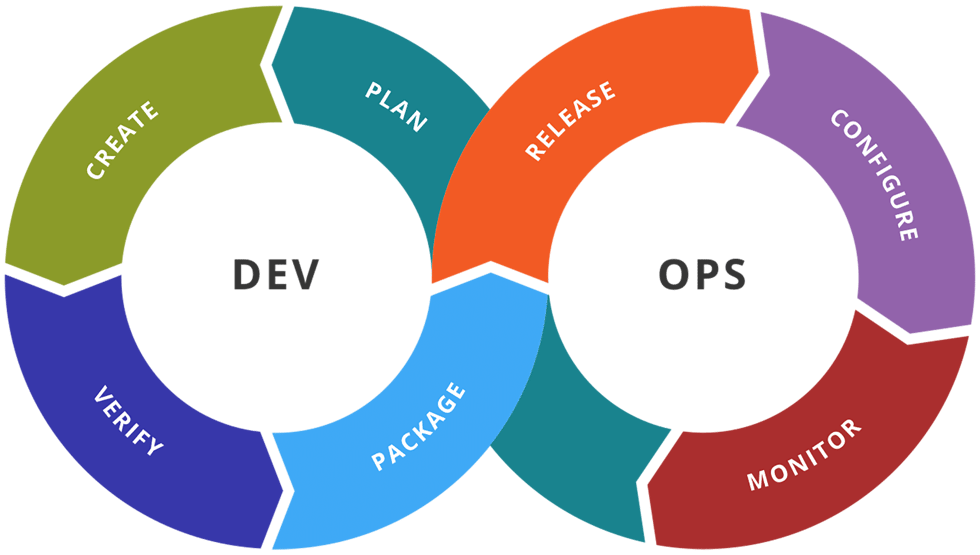
\includegraphics[width=0.6\textwidth]{img/Devops-toolchain.png}
    \caption{Fasi del ciclo di sviluppo software con tecniche DevOps}
\end{figure}

\subsection{Continuous Integration}
\label{ci-sec}
Maggiore è la complessità di un progetto e maggiore è la necessità di integrare frequentemente e preventivamente i componenti software al fine di verificare che essi funzionino correttamente~\cite{duvall2007continuous}. Con Continuous Integration (CI) si intende una pratica di sviluppo software dove i membri di un team integrano frequentemente il loro lavoro e ogni integrazione è testata e verificata da un sistema automatico in grado di intercettare gli errori il più velocemente possibile\footnote{\href{https://martinfowler.com/articles/continuousIntegration.html}{https://martinfowler.com/articles/continuousIntegration.html}}.

Con pipeline si intende una sequenza ordinata di elaborazioni che vengono applicate al codice sorgente in modo automatico. Solitamente una pipeline di CI prevede tre task:

\begin{itemize}
    \item \textbf{Build} - Il primo task consiste nella verifica della corretta compilazione del codice sorgente.
    \item \textbf{Test} - Successivamente si eseguono i task di testing, tipicamente riguardanti la logica applicativa (unit testing).
    \item \textbf{Package} - Lo scopo dell'ultimo task della pipeline di CI consiste nella verifica della corretta pacchettizzazione del codice. Deve essere possibile creare correttamente l'artefatto che verrà poi passato alle fasi successive di rilascio (delivery).
\end{itemize}

\begin{figure}[H]
    \centering
    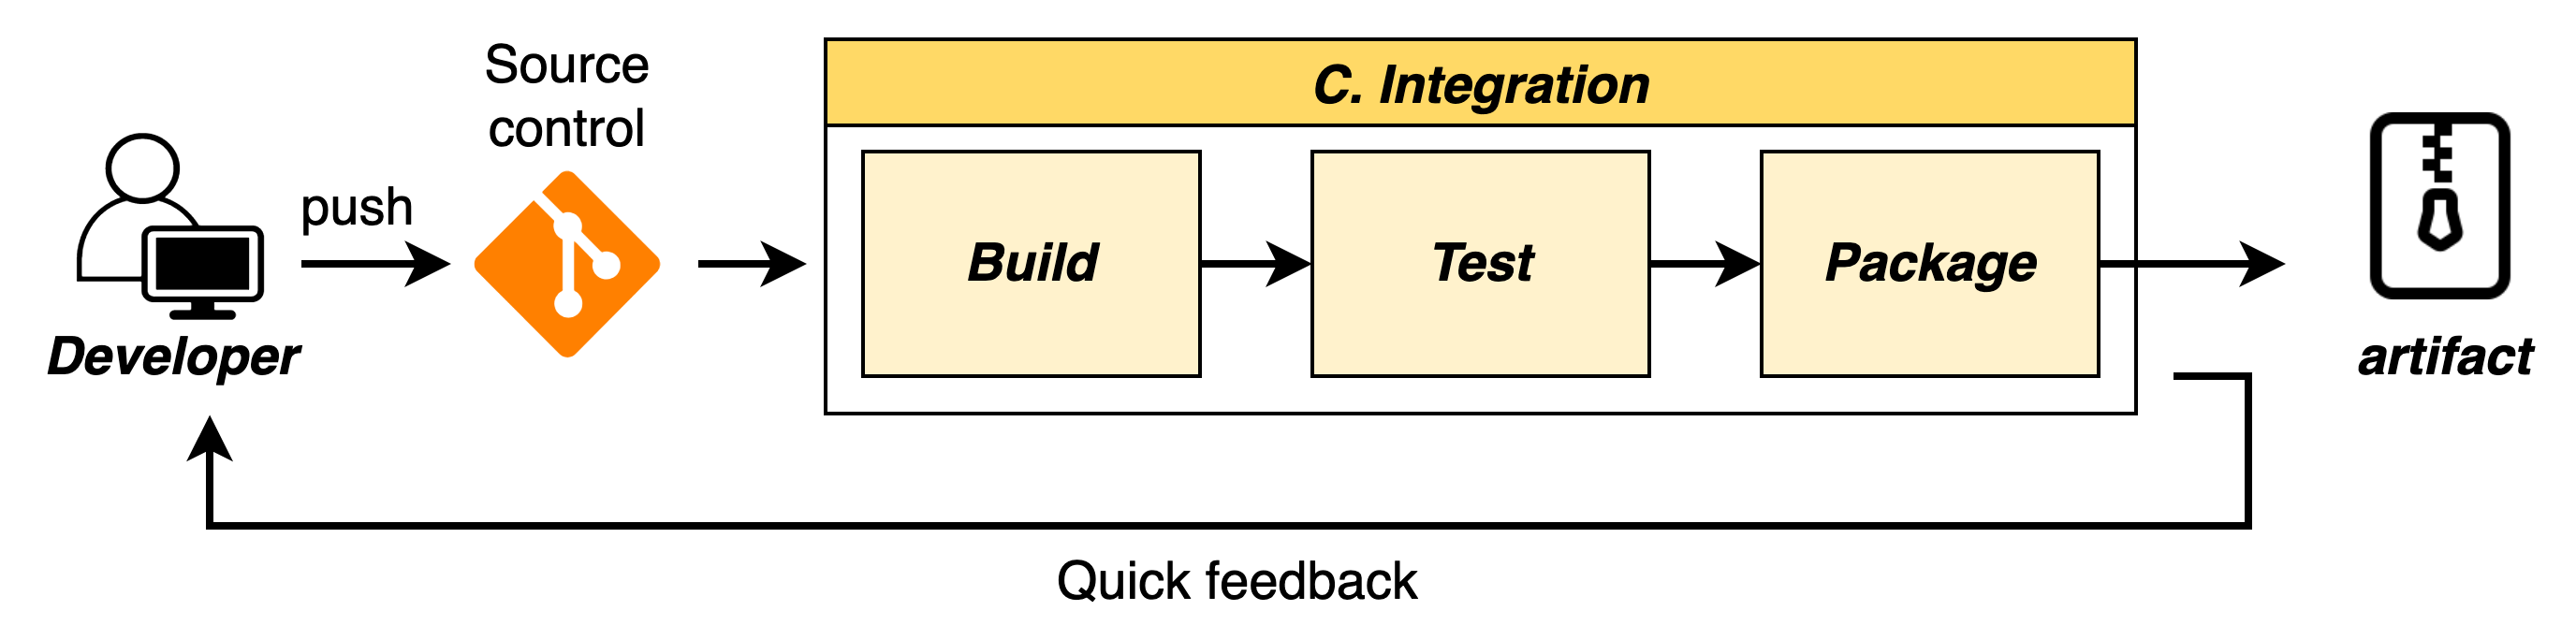
\includegraphics[width=1\textwidth]{img/ci-pipeline.png}
    \caption{Pipeline di Continuous Integration}
    \label{ci-pipeline}
\end{figure}

Ogni sviluppatore lavora effettuando piccole modifiche al codice (commit) che possono essere facilmente sistemate in caso di errori: maggiore è la modifica applicata al codice e maggiore è il rischio di problemi. Grazie ai sistemi di versionamento del codice (VCS\footnote{Version Control System}) e alle funzionalità che forniscono come branch, commit, pull request e code review gli sviluppatori possono collaborare sul codice. Unendo le funzionalità dei VCS con le funzionalità di altri sistemi appositi per l'automazione di task, come GitLab CI, GitHub Actions e Travis CI è possibile adottare efficacemente le tecniche di CI nel processo di sviluppo. Tali strumenti a supporto dei sistemi di automazione sono descritti in modo dettagliato nella sezione \ref{devops-tools-sec} di questo capitolo.

\subsection{Continuous Delivery}
\label{cd-sec}
Quando la fase di CI termina con successo si continua con la fase successiva di rilascio automatico del codice. Con Continuous Delivery (CD) si intende una pratica di sviluppo dove il software viene sviluppato in una maniera tale da poter essere installato nell'ambiente di produzione in qualsiasi momento\footnote{\href{https://martinfowler.com/bliki/ContinuousDelivery.html}{https://martinfowler.com/bliki/ContinuousDelivery.html}}. Questo significa che gli stessi concetti di (\textit{i}) piccole modifiche e (\textit{molto frequentemente}) applicati alla fase di integrazione vengono applicati anche alla fase di rilascio.

Il compito principale della fase di CD è quello di prendere il software impacchettato nell'ultimo task della fase di CI (package) e renderlo disponibile alla fase successiva di installazione (deployment) tramite la pubblicazione su appositi sistemi chiamati package manager.

\begin{figure}[H]
    \centering
    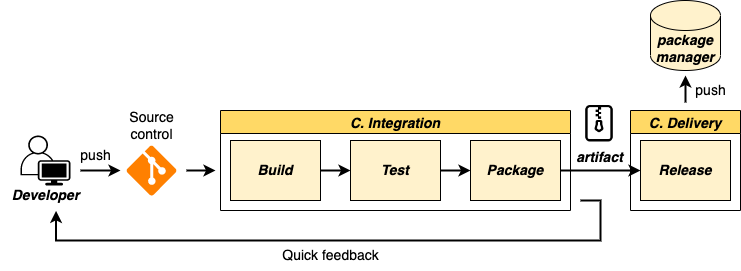
\includegraphics[width=1\textwidth]{img/cd-pipeline.png}
    \caption{Pipeline di Continuous Delivery}
    \label{cd-pipeline}
\end{figure}

I package manager devono fornire lo spazio necessario alla archiviazione dei pacchetti creati durante la fase di CI e pubblicati durante la fase di CD ma devono anche supportare altre funzionalità come versionamento dei pacchetti, diverse tipologie di pacchetto e autenticazione per il caricamento/scaricamento dei pacchetti in caso di package manager privati. Alcuni esempi di package manager sono Nexus, Maven Central Repository e NPM.

E' fondamentale che il pacchetto pubblicato sul package manager sia dato come output dalla fase di CI in modo da garantire che il codice sorgente ha passato con successo tutti i task di controllo e verifica. Lo stesso pacchetto sarà poi utilizzato nella fase successiva per l'installazione in un ambiente d'esecuzione. 

\subsection{Continuous Deployment}
In base alla natura del software che si sviluppa il processo potrebbe terminare con la fase di delivery, come ad esempio nel caso di librerie e applicazioni mobile oppure continuare con l'installazione del prodotto in un ambiente di esecuzione, come nel caso di applicazioni web e microservizi. 

Nel caso in cui sia necessaria l'installazione del prodotto in un ambiente, la fase di deployment recupera il pacchetto pubblicato in fase di delivery e lo installa. Infatti, non può esistere continuous deployment senza continuous delivery, ma non è vero il contrario.

Con Continuous Deployment si intende quindi una estensione della continuous delivery con un processo che automatizza l'intera pipeline dal momento in cui lo sviluppatore modifica il codice alla installazione di quella modifica nell'ambiente di staging o produzione~\cite{krief2019learning}.

\begin{figure}[H]
    \centering
    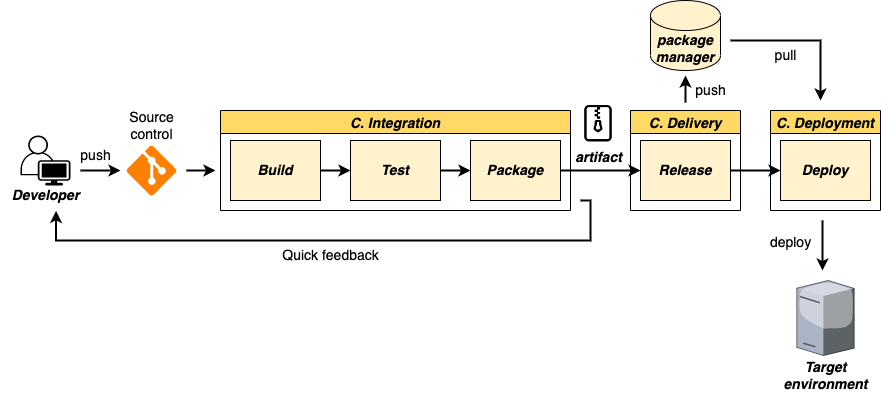
\includegraphics[width=1\textwidth]{img/cdeploy-pipeline.png}
    \caption{Pipeline di Continuous Deployment}
    \label{cdeploy-pipeline}
\end{figure}

\subsection{Continuous Monitoring}
Poter raccogliere dati dal sistema per poterlo analizzare è uno dei punti chiave del DevOps poiché permette di migliorare sia il prodotto che il processo: garantisce integrità, prestazioni e affidabilità in ogni fase del ciclo di vita del software.

\begin{figure}[H]
    \centering
    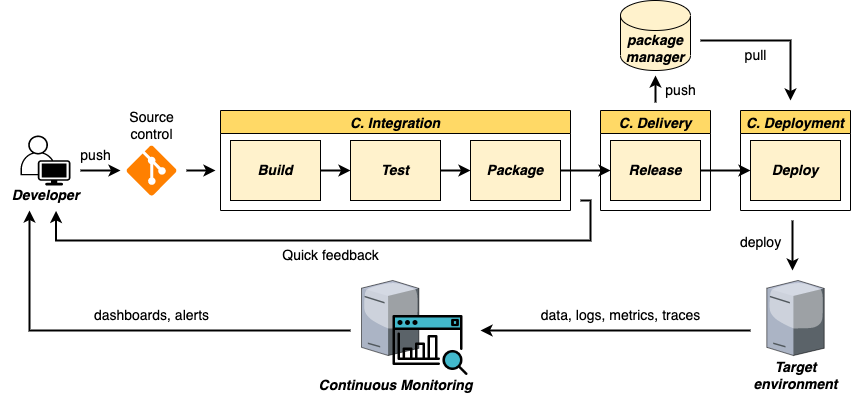
\includegraphics[width=1\textwidth]{img/ci-monitoring.png}
    \caption{Integrazione tipica di un sistema di Continuous Monitoring}
    \label{ci-monitoring}
\end{figure}

Anche la fase di monitoring deve essere continua e automatica ma a differenza della CI/CD, le pratiche di monitoraggio eseguono task che riguardano tutto il processo indipendentemente dal lavoro svolto dallo sviluppatore. Ad esempio:

\begin{itemize}
    \item raccolta di metriche riguardanti il processo di sviluppo (commit effettuate, merge request chiuse e approvate, issues, pipeline fallite, ...),
    \item raccolta di metriche riguardanti il software rilasciato (numero di download effettuati, recensioni, ...),
    \item raccolta di metriche riguardanti l'ambiente d'esecuzione del software installato (log, metriche, traces),
    \item centralizzazione di tutti i dati raccolti,
    \item invio di notifiche (alerting) al raggiungimento di una certa soglia da parte di una specifica metrica,
    \item creazione di dashboard per la visualizzazione grafica.
\end{itemize}

Lo scopo principale della pratica di continuous monitoring è ridurre il più possibile il tempo che intercorre tra il momento in cui un difetto è introdotto nel codice o nel processo, intercettato e risolto.

Le stesse pratiche si possono adottare per il monitoraggio dell'utente con l'obiettivo di raccogliere dati sul suo comportamento per migliorare l'esperienza utente, fare analisi di mercato o creare raccomandazioni. Tipicamente ci si riferisce a questa pratica con il termine analytics.

\subsection{Continuous Inspection}
Tipicamente vengono definiti a livello aziendale degli standard di qualità e di sicurezza
che devono essere rispettati da ogni team di sviluppo per qualsiasi prodotto software. La
definizione di linee guida sullo stile di programmazione o sul livello di severity accettato sono esempi di standard di qualità. La pratica di analizzare automaticamente e molto frequentemente il codice al fine di validare il rispetto degli standard di qualità e sicurezza è chiamata Continuous
Inspection.

L’obiettivo è quello di ottenere un feedback sullo stato del codice, sullo stato
del processo e sulla presenza di problemi di sicurezza al fine di pianificare interventi
risolutivi nel minor tempo possibile. Come nel caso del monitoraggio esiste un sistema terzo a supporto dei task necessari e in grado di fornire feedback allo sviluppatore. I principali task di analisi che compongono la fase di ispezione continua sono:

\begin{itemize}
    \item \textbf{Static Application Security Testing} (SAST) - Analisi white-box della applicazione al fine di individuare vulnerabilità, code smell e bug ma anche di verificare il rispetto di un certo livello di qualità.
    \item \textbf{Software Composition Analysis} (SCA) - Analisi delle dipendenze di progetto con lo scopo di individuare vulnerabilità pubbliche (CVE\footnote{Common Vulnerability and Exposure}) associate ad esse.
\end{itemize}

In entrambe le tipologie di analisi è fondamentale ottenere come risultato un report della scansione, in grado di descrivere in modo dettagliato eventuali entità individuate dalla fase di analisi. I report vengono prodotti tipicamente sia in formati human-readable (es. pagina HTML) che machine-readable (es. JSON, XML) per poter essere utilizzati da applicazioni terze come ad esempio sistemi centralizzati per la consultazione di report eterogenei chiamati Vulnerability Management System.

\begin{figure}[H]
    \centering
    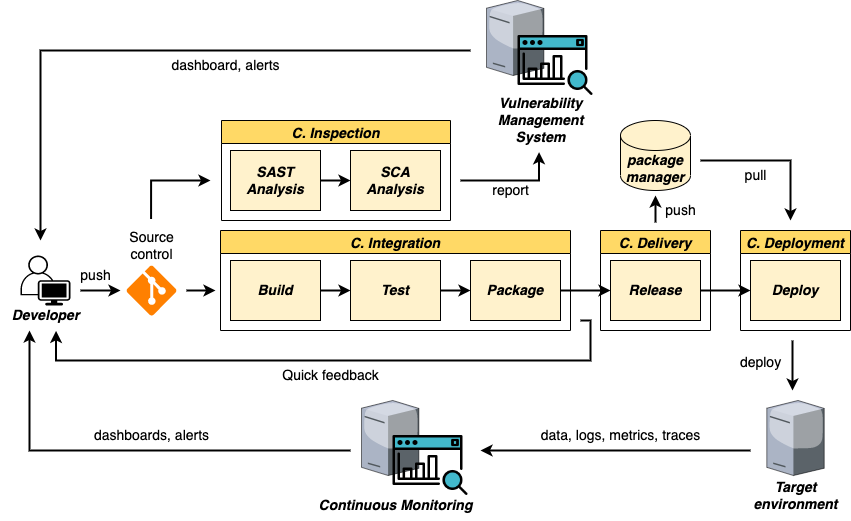
\includegraphics[width=1\textwidth]{img/cinspection-pipeline.png}
    \caption{Integrazione tipica di un sistema di Continuous Inspection}
    \label{ci-inspection-pipeline}
\end{figure}

\section{Strumenti}
\label{devops-tools-sec}
Per poter mettere in pratica le tecniche di CI/CD in modo da adottarle efficacemente nel processo di sviluppo è necessaria una infrastruttura complessa composta da tanti servizi e strumenti. Data la grande complessità soprattutto nella gestione, manutenzione e integrazione di tutti questi componenti spesso si fa uso di una o piu piattaforme cloud in modo da avere a disposizione un sistema in grado di fornire i seguenti strumenti fondamentali:
\begin{itemize}
    \item \textbf{Version Control System} - Strumento per il versionamento del codice e tracciamento delle modifiche che permette la collaborazione tra i componenti di un team. Con l'avvento delle metodologie agile e della cultura DevOps, l'uso di un VCS nei processi è diventato obbligatorio.
    \item \textbf{Package Manager} - Strumento per l'archiviazione e la condivisione del software sviluppato sotto forma di pacchetti, come descritto nella sezione \ref{cd-sec}.
    \item \textbf{CI Server} - Strumento in grado di eseguire elaborazioni in modo automatico su un server remoto e restituire il risultato. Rappresenta il motore di tutta la automazione a supporto delle tecniche CI/CD.
\end{itemize}

\subsection{Pipeline as Code}
Nella sezione \ref{ci-sec} il concetto di pipeline è stato definito come una sequenza ordinata di elaborazioni che vengono applicate al codice sorgente in modo automatico. In realtà una pipeline di CI/CD è suddivisa in più passi, detti stage, i quali contengono una o più elaborazioni, dette job.

Lo strumento adottato da quasi tutte le principali piattaforme per la definizione degli stage e dei job che compongono una pipeline e quindi per istruire un CI Server all'esecuzione effettiva dei task è chiamato Pipeline as Code. Questo metodo permette di descrivere il processo di una pipeline in un file testuale, tipicamente in formato YAML, che si trova nello stesso repository in cui risiede il codice sorgente.

Il seguente codice\footnote{\href{https://github.com/paganellif/DevOps-per-applicazioni-mobile-un-caso-di-studio-industriale/blob/1-metodologia-devops/.gitlab-cy.yml}{https://github.com/paganellif/DevOps-per-applicazioni-mobile-un-caso-di-studio-industriale/blob/1-metodologia-devops/.gitlab-cy.yml}} contiene la definizione di una pipeline descritta utilizzando la sintassi per la piattaforma specifica GitLab. In questo caso la pipeline è composta da due stage (\textit{build} e \textit{deploy}), ognuno dei quali contiene a sua volta un job. Il cuore del job, ovvero le istruzioni bash che il CI Server deve eseguire sono definite tramite la keyword \textit{script}.

\begin{listing}[H]
    \inputminted{yaml}{code/3-pipelineexample}
    \caption{Pipeline d'esempio per la piattaforma GitLab}
\end{listing}

I vantaggi derivanti dall'utilizzo del meccanismo Pipeline as Code sono:
\begin{itemize}
    \item versionamento dei file che descrivono le pipeline di CI/CD in modo da tracciare anche le modifiche che vengono apportate al processo automatizzato,
    \item utilizzo di metodologie simili a quelle utilizzate nello sviluppo software (ereditarietà, incapsulamento, riuso, ...),
    \item i file che descrivono il processo sono accessibile a tutto il team ed è possibile collaborare alla sua modifica in modo identico allo sviluppo software.
\end{itemize}

\subsection{Runners}
L'architettura di un CI Server deve essere costruita in modo robusto e scalabile per poter supportare efficacemente le tecniche CI/CD. Basta un team con un numero minimo di sviluppatori e un numero minimo di progetti ai quali sono applicate le tecniche CI/CD e la metodologia di sviluppo agile per comprendere l'enorme quantità di lavoro a cui un CI Server può essere sottoposto.

Ogni evento che si verifica sulla piattaforma in cui è mantenuto il codice sorgente viene intercettato dal CI Server: se nel file che descrive la pipeline è definito un job in associazione a quello specifico evento, il CI Server invia tutte le informazioni utili per l'esecuzione del job ad un altro componente software chiamato runner e rimane in attesa del risultato. 

\begin{figure}[H]
    \centering
    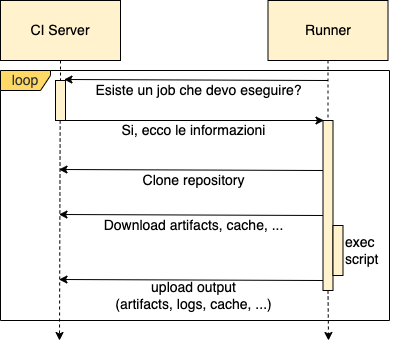
\includegraphics[width=0.65\textwidth]{img/ciserver-runner.png}
    \caption{Diagramma di sequenza interazione CI Server-Runner}
    \label{ci-server-runner}
\end{figure}

Il runner consiste in un componente architetturale della infrastruttura che necessita di un ambiente di esecuzione e per svolgere il suo compito consuma delle risorse. In base a chi lo gestisce il runner può essere:

\begin{itemize}
    \item \textbf{Managed} - Funzionalità fornita as-a-Service dalla piattaforma che si utilizza. In base al piano di licenza sottoscritto con la piattaforma l'utilizzo dei runner è soggetto a limiti che riguardano tipicamente i minuti di utilizzo e lo spazio di archiviazione. Il vantaggio di questa modalità è che non è richiesto alcuno sforzo nella configurazione e manutenzione del runner e nessuna spesa per l'ambiente di esecuzione.
    \item \textbf{Self-Hosted} - Il componente è gestito dall'utilizzatore in tutti i suoi aspetti ma non è soggetto ad alcun tipo di vincolo in termini di risorse utilizzate.
\end{itemize}

\clearpage{\pagestyle{empty}\cleardoublepage}
\chapter{Mobile Application Development Lifecycle}
\label{ch:sdlc}
% !TeX root = ../main.tex

\section{Introduzione}
In questo capitolo viene analizzato il processo di sviluppo tipico per le applicazioni mobile al fine di porre le basi per la progettazione dello stesso processo di sviluppo applicando pratiche e tecniche DevOps di automazione. Lo scopo di questa fase iniziale di progetto è quindi la definizione di tutti i principali task e sotto-task necessari allo sviluppo di applicazioni mobile, dalla scrittura del codice sorgente al rilascio sui marketplace delle relative piattaforme target.

Il processo di sviluppo delle applicazioni mobile è simile a quello di qualsiasi altra applicazione software: in questo caso l'obiettivo è distribuire l'applicazione al fine di dare la possibilità all'utente di installarla sul proprio dispositivo, mentre tipicamente nei processi di altre tipologie di applicazioni, come per esempio le Web Application, l'obiettivo è quello di mettere in esecuzione l'applicazione in un ambiente target accessibile all'utente tramite la rete.

A prescindere dalla tipologia di applicazione, il processo di sviluppo è composto concettualmente dalla stessa sequenza di fasi di lavoro: (\textit{i}) pianificazione, (\textit{ii}) progettazione, (\textit{iii}) sviluppo, (\textit{iv}) stabilizzazione, (\textit{v}) rilascio e (\textit{vi}) monitoraggio. Ognuna di queste macro-fasi comprende a sua volta una serie di sotto-fasi tra le quali esistono specifiche dipendenze:

\begin{figure}[H]
    \centering
    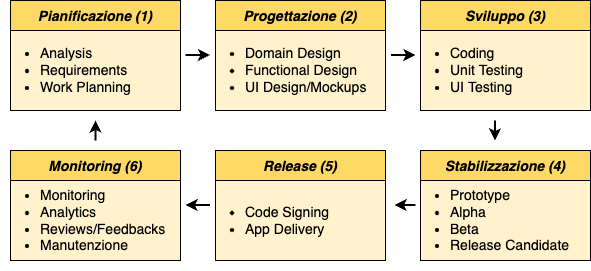
\includegraphics[width=0.7\textwidth]{img/sdlc.png}
    \caption{Ciclo di vita di sviluppo tipico delle applicazioni mobile.}
    \label{sdlc-app-mobile-fig}
\end{figure}

\section{Pianificazione}
In questa prima fase del processo di sviluppo si formalizzano i requisiti, funzionali e non funzionali, che devono essere soddisfatti dalla applicazione per ottenere l'approvazione del committente e si pianifica il lavoro per le successive fasi in termini di task, risorse e tempo.

Tramite la definizione di casi d'uso si rappresentano le interazioni tra il sistema e dei ruoli (attori in UML\footnote{Unified Modeling Language}) necessarie al raggiungimento di un obiettivo. Questi casi d'uso sono dunque dei possibili scenari dove il sistema riceve delle richieste esterne, come l'input dell'utente, e risponde ad esso. Dopo aver acquisito un numero appropriato di casi d'uso e attori è molto più semplice iniziare a progettare una applicazione. Lo sviluppo può quindi concentrarsi su come creare l'applicazione anziché sulla sua definizione o la sua funzione.

\section{Progettazione}
La fase di progettazione della applicazione è composta da un insieme di sottotask tra cui la modellazione del dominio applicativo, la scelta della architettura da utilizzare e la prototipazione dell'esperienza utente e dell'interfaccia grafica (UX/UI).

Tipicamente la progettazione UX/UI viene svolta tramite l'ausilio di mockup per definire prima come l'utente intende utilizzare l'applicazione (esperienza) e poi aspetti grafici come colori, font e icone (interfaccia).

\section{Sviluppo}
Una volta progettata l'applicazione è possibile partire con la fase di sviluppo. Solitamente l'obiettivo è far iniziare la fase di sviluppo il prima possibile in modo da sviluppare un prototipo funzionante ed ottenere la validazione da parte del committente, la quale è l'obiettivo principale della fase successiva.

\section{Stabilizzazione}
La stabilizzazione consiste nella risoluzione di problemi sia a livello funzionale che a livello di usabilità e di prestazioni al fine di ottenere una versione di applicazione pronta da distribuire. Questa parte del ciclo di sviluppo dovrebbe iniziare il più presto possibile in modo da individuare e risolvere i problemi prima che diventino un costo. Tipicamente per qualsiasi applicazione, anche non specifica per i dispositivi mobile, sono previste le seguenti sottofasi del processo di stabilizzazione\footnote{\href{https://docs.microsoft.com/itit/xamarin/cross-platform/get-started/introduction-to-mobile-sdlc}{https://docs.microsoft.com/itit/xamarin/cross-platform/get-started/introduction-to-mobile-sdlc}}:
\begin{itemize}
    \item \textbf{Prototype} - L'applicazione include soltanto alcune delle funzionalità principali e sono presenti bug maggiori. In questa fase il focus è sulla singola funzionalità implementata fornita dal prototipo per il testing.
    \item \textbf{Alpha} - Tutte le principali funzionalità sono completate e devono essere testate.
    \item \textbf{Beta} - Gran parte delle funzionalità, sia principali che ausiliarie, sono state completate e i bug maggiori sono stati risolti.
    \item \textbf{Release Candidate} - Tutte le funzionalità sono state completate e testate, ma potrebbero essere presenti ancora bug minori.
\end{itemize}

\subsection{Alpha}
La prima versione funzionante di una applicazione è detta alpha ed è utilizzata per il testing interno di specifiche funzionalità. Questo significa che può presentare anche bug o funzionalità mancanti ma almeno deve contenere le funzionalità che devono essere testate per quella specifica versione alpha.

Solitamente prima della release di una applicazione, anche se in fase di testing, è necessario attendere la sua approvazione da parte del gestore del servizio. Il processo di approvazione pre-release è detto \textit{App Review}. Nel caso del testing interno è possibile distribuire la applicazione ad un insieme ristretto di tester.

Continuando con i rilasci di versioni alpha vengono aggiunte nuove funzionalità e/o risolti eventuali bug: quando la versione è considerata pronta viene eseguita una sua promozione. Con promozione si intende in questo caso il rilascio di una versione alpha in versione beta.

\subsection{Beta}
A questo punto del processo di sviluppo la applicazione è considerata completa a tutti gli effetti a meno di bug e/o problemi di stabilità. La versione beta rappresenta dunque la prima versione della applicazione resa disponibile ai tester esterni, ovvero quegli utenti che non hanno partecipato alle fasi di sviluppo e che svolgono il ruolo di validazione delle funzionalità. Si distinguono due tipologie di beta testing:
\begin{itemize}
    \item \textit{Aperto} - La applicazione è rilasciata per la fase di testing esterno permettendo l'accesso a qualsiasi utente con account da beta tester. Nel caso di Android per poter testare una applicazione in versione beta aperta è necessario disporre di un account Google Developer.
    \item \textit{Chiuso} - L'accesso alla applicazione di test è limitato ad un insieme ristretto di tester, tipicamente gestiti tramite mailing list o link di condivisione.
\end{itemize}
Dopo aver ottenuto la validazione da parte dei tester, la quale potrebbe richiedere più iterazioni di sviluppo e rilascio di versioni alpha-beta, anche per la versione beta si effettua la promozione, rilasciando la applicazione in produzione.

\section{Release}
Dopo che la applicazione è stata stabilizzata è possibile procedere con la distribuzione. In questa fase l'applicazione viene prima firmata digitalmente utilizzando un certificato protetto da chiave privata e poi pubblicata sullo specifico marketplace della piattaforma target.

\section{Monitoraggio}
La fase di monitoraggio (e manutenzione) è quella più lunga e dispendiosa in termini di tempo e risorse. Per le applicazioni mobile esistono alcune situazioni che rendono il monitoraggio più complesso rispetto ad altre tipologie di applicazioni come ad esempio le web app. Bisogna infatti considerare che\footnote{\href{https://www.datadoghq.com/blog/mobile-monitoring-best-practices/}{https://www.datadoghq.com/blog/mobile-monitoring-best-practices/}}:
\begin{itemize}
    \item le applicazioni mobile eseguono su una vasta gamma di dispositivi con caratteristiche diverse e può essere quindi difficile ottenere una chiara visibilità delle prestazioni lato client;
    \item se gli utenti riscontrano un problema, mentre una patch per applicazioni web può essere distribuita quasi all'istante, la distribuzione degli aggiornamenti delle applicazioni mobile richiede tempo e l'attivazione da parte degli utenti per scaricarli.
\end{itemize}
Per effettuare un monitoraggio efficace è necessario misurare e controllare continuamente le performance della applicazione mobile, il comportamento dell'utente e gli errori che essi riscontrano. Alcuni esempi di metriche fondamentali sono: tempo di avvio della applicazione, network performance, utilizzo delle risorse (CPU, disco e memoria) e metriche custom derivanti dalle azioni dell'utente.

\clearpage{\pagestyle{empty}\cleardoublepage}
\chapter{Applicazioni Multipiattaforma}
\label{ch:app-multiplatform}
% !TeX root = ../main.tex

\section{Introduzione}
La continua crescita della quantità di dispositivi mobile presenti, e in particolare gli smartphone, ha reso molto importante a livello globale il mercato delle applicazioni e per questo motivo sono sempre di più le aziende che decidono di investire risorse nello sviluppo e nella vendita di applicazioni mobile. Una azienda che intende targettizzare il maggior numero di utenti possibile con le proprie applicazioni deve considerare che l'intero mercato è spartito in base alla diffusione dei sistemi operativi per smartphone. Ad oggi, i sistemi operativi più diffusi sono Android (Google) e iOS (Apple), i quali coprono quasi la totalità del mercato con quote rispettivamente del 71\% e del 28\%\footnote{\href{https://www.statista.com/statistics/272698/global-market-share-held-by-mobile-operating-systems-since-2009/}{https://www.statista.com/statistics/272698/global-market-share-held-by-mobile-operating-systems-since-2009/}}. Questi dati comportano per una azienda la necessità di sviluppare la stessa applicazione per almeno due piattaforme completamente differenti tra loro. A tal proposito sono nate nuove metodologie e tecniche basate sul concetto "Write Once, Run Anywhere" (WORA)\footnote{\href{https://www.computerweekly.com/feature/Write-once-run-anywhere}{https://www.computerweekly.com/feature/Write-once-run-anywhere}} con lo scopo di ottimizzare lo sviluppo delle applicazioni mobile al fine di ridurre i costi e aumentare l'efficienza del processo di sviluppo.

Le principali tecniche moderne di sviluppo per applicazioni mobile sono:
\begin{itemize}
    \item \textbf{Cross-platform} - Rispetta completamente la filosofia WORA. Lo stesso codice può essere eseguito su diverse piattaforme grazie ad uno strato applicativo aggiuntivo che si occupa di interpretare il codice e tradurlo nel linguaggio specifico della piattaforma target.
    \item \textbf{Multi-platform} - Tecnica più recente che permette di sviluppare applicazioni native condividendo solamente la logica applicativa. In questo caso non è necessario uno strato software aggiuntivo perchè la applicazione può essere eseguita direttamente dalla piattaforma target.
\end{itemize}

\section{Cross-platform vs Multi-platform}
Sia nel caso cross-platform che nel caso multi-platform i principali vantaggi, che sono la riduzione dei costi e l'ottimizzazione del processo di sviluppo, derivano dalla condivisione e dal riuso del codice e quindi meno risorse impiegate rispetto allo sviluppo classico delle applicazioni mobile native.

Esistono però alcune differenze tra loro, fondamentali durante la scelta della metodologia da adottare da parte di una azienda per lo sviluppo di una applicazione mobile.
\begin{itemize}
    \item \textbf{Cross-platform}
    \begin{itemize}
        \item Condivisione/riuso totale del codice. Sia la logica applicativa che l'interfaccia utente sono le stesse per qualsiasi piattaforma.
        \item Performance limitate rispetto al nativo, dovute dalla presenza di uno strato software aggiuntivo che interpreta e traduce il codice.
        \item Accesso alle funzionalità hardware del dispositivo limitato e/o con overhead, dovuto sempre dalla presenza dello strato software aggiuntivo.
    \end{itemize}
    \item \textbf{Multi-platform}
    \begin{itemize}
        \item Condivisione/riuso della sola logica applicativa. Lo sviluppo dell'interfaccia utente rimane nativo.
        \item Performance elevate, equivalenti a quelle native.
        \item Accesso completo e senza overhead a tutte le funzionalità hardware del dispositivo.
    \end{itemize}
\end{itemize}

\section{Strumenti}
\label{app-multiplatform-tools}
Tipicamente quando ci si approccia allo sviluppo di una qualsiasi tipologia di software si effettua una ricerca di tutti gli strumenti in grado di facilitare il lavoro dello sviluppatore. Le principali categorie di strumenti necessari sono: (\textit{i}) linguaggio di programmazione, (\textit{ii}) ambiente di sviluppo (IDE\footnote{Integrated Development Environment}), (\textit{iii}) build automation e (\textit{iv}) framework di sviluppo.

La scelta di questi strumenti è spesso vincolata dalla piattaforma target, ovvero l'ambiente dove eseguirà il codice, e lo è in particolare per le applicazioni mobile. A differenza dello sviluppo di applicazioni Android, dove gran parte degli strumenti più diffusi è open-source, lo sviluppo di applicazioni iOS richiede vincoli stringenti imposti da Apple come ad esempio l'utilizzo dell'IDE XCode, il quale è disponibile solamente per il sistema operativo macOS.

Per gli strumenti di build automation esistono diverse alternative per l'ecosistema Android, anche se lo standard de-facto è dato dal tool Gradle. Lo stesso non è vero invece per le applicazioni iOS: come per l'IDE anche in questo caso è necessario utilizzare un insieme di tool specifici indicati da Apple. I più popolari frameworks open-source per lo sviluppo di applicazioni cross-platform sono: (\textit{i}) Ionic, (\textit{ii}) Flutter e (\textit{iii}) React Native. Il paradigma multi-platform è più recente rispetto al quello cross-platform e il principale framework open-source in questo caso è Kotlin Multiplatform.

\subsection{Kotlin Multiplatform Mobile}
Kotlin Multiplatform Mobile\footnote{\href{https://kotlinlang.org/lp/mobile/}{https://kotlinlang.org/lp/mobile/}} (KMM) è un framework per lo sviluppo di applicazioni Android e iOS basato sul concetto di condivisione della logica applicativa mantenendo lo sviluppo nativo della UX/UI.

\begin{figure}[H]
    \centering
    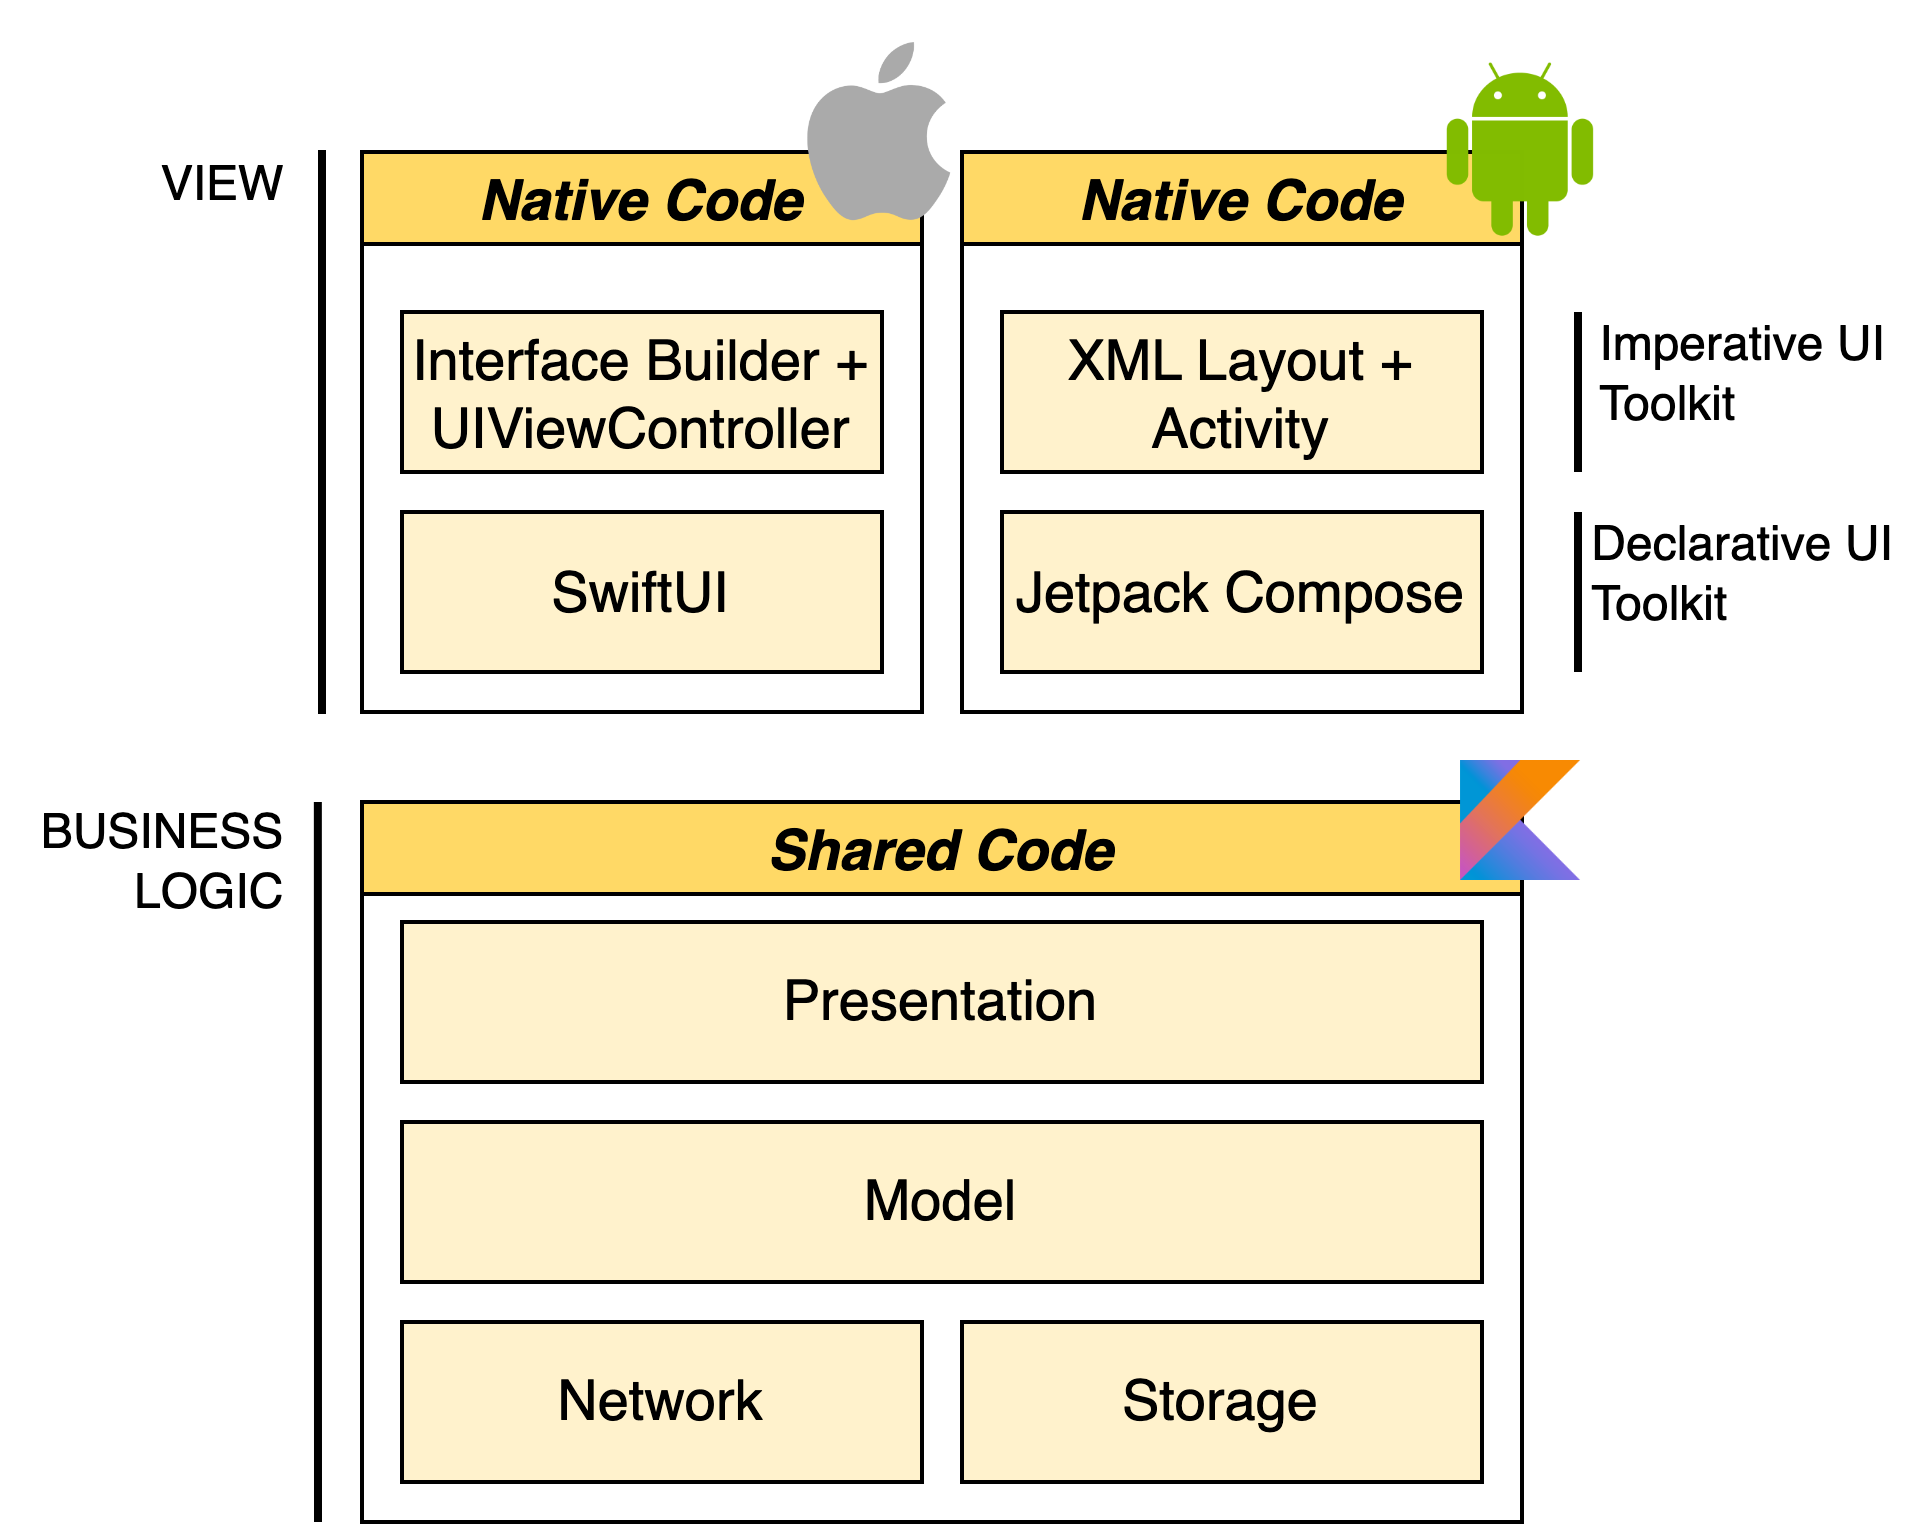
\includegraphics[width=0.7\textwidth]{img/stack_kmm.png}
    \caption{Stack architetturale Kotlin Multiplatform Mobile.}
    \label{stackKMM}
\end{figure}

Con il rilascio di Kotlin 1.7.20 (Settembre 2022), KMM è passato dalla fase \textit{Alpha} alla fase \textit{Beta} la quale è considerata come fase "\textit{pre-stable}"\footnote{\href{https://kotlinlang.org/docs/components-stability.html\#current-stability-of-kotlin-components}{https://kotlinlang.org/docs/components-stability.html\#current-stability-of-kotlin-components}} ma è comunque già stato adottato in produzione per lo sviluppo delle proprie applicazioni mobile da tante aziende tra le quali è possibile trovare nomi rilevanti come Netflix, VMware e Philips\footnote{\href{https://kotlinlang.org/lp/mobile/case-studies/}{https://kotlinlang.org/lp/mobile/case-studies/}}. In base al risultato dell'indagine di mercato svolta nei primi due quadrimestri del 2021\footnote{\href{https://blog.jetbrains.com/kotlin/2021/10/multiplatform-survey-q1-q2-2021/}{https://blog.jetbrains.com/kotlin/2021/10/multiplatform-survey-q1-q2-2021/}}, le porzioni di codice condiviso nelle applicazioni sviluppate con KMM sono: 85\% networking, 75\% data storage, 70\% utilities, $\sim$60\% algoritmi/computazione, $\sim$55\% state management e $\sim$50\% presenters/controllers/view models.

KMM consiste in un caso d'uso specifico (e il più diffuso) del framework Kotlin MultiPlatform (KMP), il quale permette di sviluppare il codice in modo agnostico rispetto le piattaforme target e di condividerlo tra differenti piattaforme. Il framework KMM è fortemente basato sui seguenti compilatori inclusi nell'ecosistema Kotlin~\cite{nagy2022simplifying}:

\begin{itemize}
    \item \textbf{Kotlin/JVM} - Utilizzato per la piattaforma Android, permette di compilare codice Kotlin in bytecode Java (\textit{.class}), il quale può essere eseguito direttamente sulla JVM. Nel caso di Android è necessario un ulteriore passaggio per tradurre il bytecode Java in bytecode Dalvik (\textit{.dex}).

    \begin{figure}[H]
        \centering
        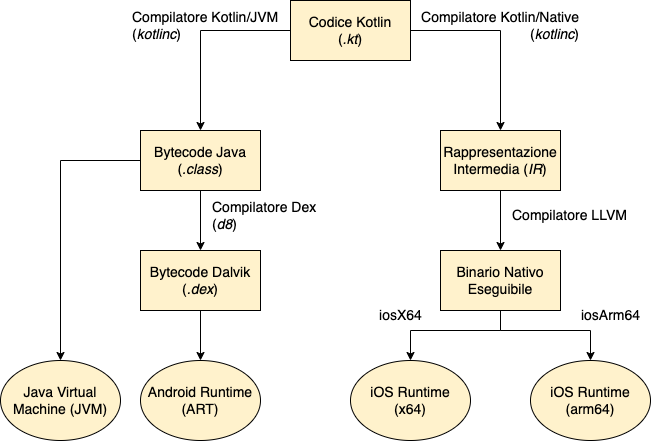
\includegraphics[width=0.8\textwidth]{img/compilatore_kotlin.png}
        \caption{Fasi di compilazione Kotlin/JVM e Kotlin/Native.}
    \end{figure}

    \item \textbf{Kotlin/Native} - Utilizzato per la piattaforma iOS. A differenza del compilatore Kotlin/JVM, il compilatore Kotlin/Native è progettato per quelle situazioni dove non è possibile o non si vuole avere una VM come nel caso dei dispositivi embedded e della piattaforma iOS. Per fare ciò include un backend basato su \textit{Low Level Virtual Machine} (LLVM)\footnote{\href{https://llvm.org/}{https://llvm.org/}} in grado di compilare il codice Kotlin in binari nativi che possono essere eseguiti senza VM\cite{nagy2022simplifying}. Le piattaforme supportate da Kotlin/Native attualmente sono macOS, iOS, tvOS, watchOS, Linux, Windows (MinGW) e Android NDK\footnote{\href{https://kotlinlang.org/docs/native-overview.html\#target-platforms}{https://kotlinlang.org/docs/native-overview.html\#target-platforms}} e per ognuna di esse esistono differenti architetture. Nel caso di iOS le differenti architetture supportate da KMM sono \textit{Arm64}, \textit{Arm32} e \textit{x64}. Anche in questo caso sono necessarie due fasi di compilazione: (\textit{i}) il codice Kotlin viene compilato nella \textit{Rappresentazione Intermedia} (IR) LLVM e (\textit{ii}) successivamente compilato nel binario nativo.
\end{itemize}

\subsubsection{Struttura Applicazione KMM}
Una applicazione sviluppata con KMM segue lo stack definito dalla condivisione della business logic e la separazione della UX/UI (figura \ref{stackKMM}). Il modulo \textit{shared} contiene tutta la business logic condivisa, la quale può essere sviluppata tramite l'utilizzo di librerie con supporto nativo al framework KMM, cioè librerie che forniscono già al loro interno specifiche implementazioni per le diverse piattaforme target, oppure tramite l'utilizzo del meccanismo expect/actual.

\begin{figure}[H]
    \centering
    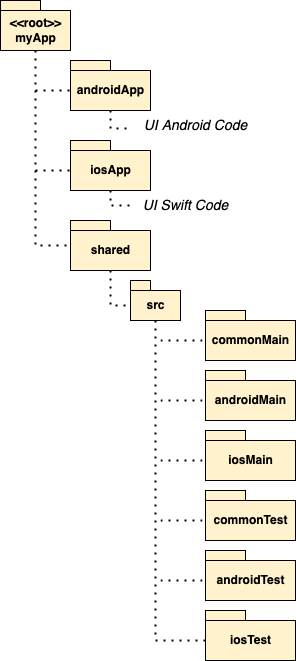
\includegraphics[width=0.5\textwidth]{img/struttura_app_kmm.png}
    \caption{Struttura dei moduli di una applicazione KMM.}
\end{figure}

Nel caso di utilizzo del meccanismo expect/actual è necessario definire le funzionalità nel modulo \textit{commonMain} e fornire le implementazioni per le specifiche piattaforme nei relativi moduli \textit{androidMain} e \textit{iosMain}. Gli stessi concetti vengono applicati per la struttura dei moduli di test: \textit{commonTest}, \textit{androidTest} e \textit{iosTest}.

I moduli UX/UI delle relative piattaforme includono il codice condiviso come dipendenza di progetto, in particolare come dipendenza Gradle (\textit{aar}\footnote{Android Archive}) per Android e come dipendenza CocoaPods (Pod) per iOS.

\subsubsection{Expect/Actual}
Quando si sviluppa codice condiviso è spesso necessario definire come determinate funzionalità debbano essere implementate sulla specifica piattaforma target per utilizzare i relativi SDK. Il framework KMM fornisce il meccanismo \textit{expect/actual} per assolvere a questo compito in modo del tutto analogo al design pattern \textit{Template Method}:
\begin{itemize}
    \item \textbf{Expect} - Astrazione della funzionalità necessaria. Tramite la keywork \textit{expect} si definisce lo scheletro astraendo dalla specifica implementazione.
    \item \textbf{Actual} - Implementazione specifica per una determinata piattaforma. Tramite la keywork \textit{actual} si definisce l'implementazione, reificando l'astrazione definita tramite il concetto di \textit{expect}.
\end{itemize}

Il seguente codice\footnote{\href{https://github.com/paganellif/DevOps-per-applicazioni-mobile-un-caso-di-studio-industriale/tree/3-applicazioni-multipiattaforma/kmm-example/shared}{https://github.com/paganellif/DevOps-per-applicazioni-mobile-un-caso-di-studio-industriale/tree/3-applicazioni-multipiattaforma/kmm-example/shared}} mostra un esempio elementare di utilizzo del meccanismo:

\begin{listing}[H]
    \inputminted{kotlin}{code/3-expectactual}
    \caption{Esempio di applicazione expect/actual per ottenere informazioni sulla piattaforma.}
\end{listing}

I seguenti screenshot, catturati tramite l'esecuzione degli appositi emulatori delle piattaforme target, mostrano l'efficacia del meccanismo expect/actual: l'applicazione è stata compilata utilizzando le differenti implementazioni in modo corretto.

\begin{multicols}{2}
    \begin{figure}[H]
        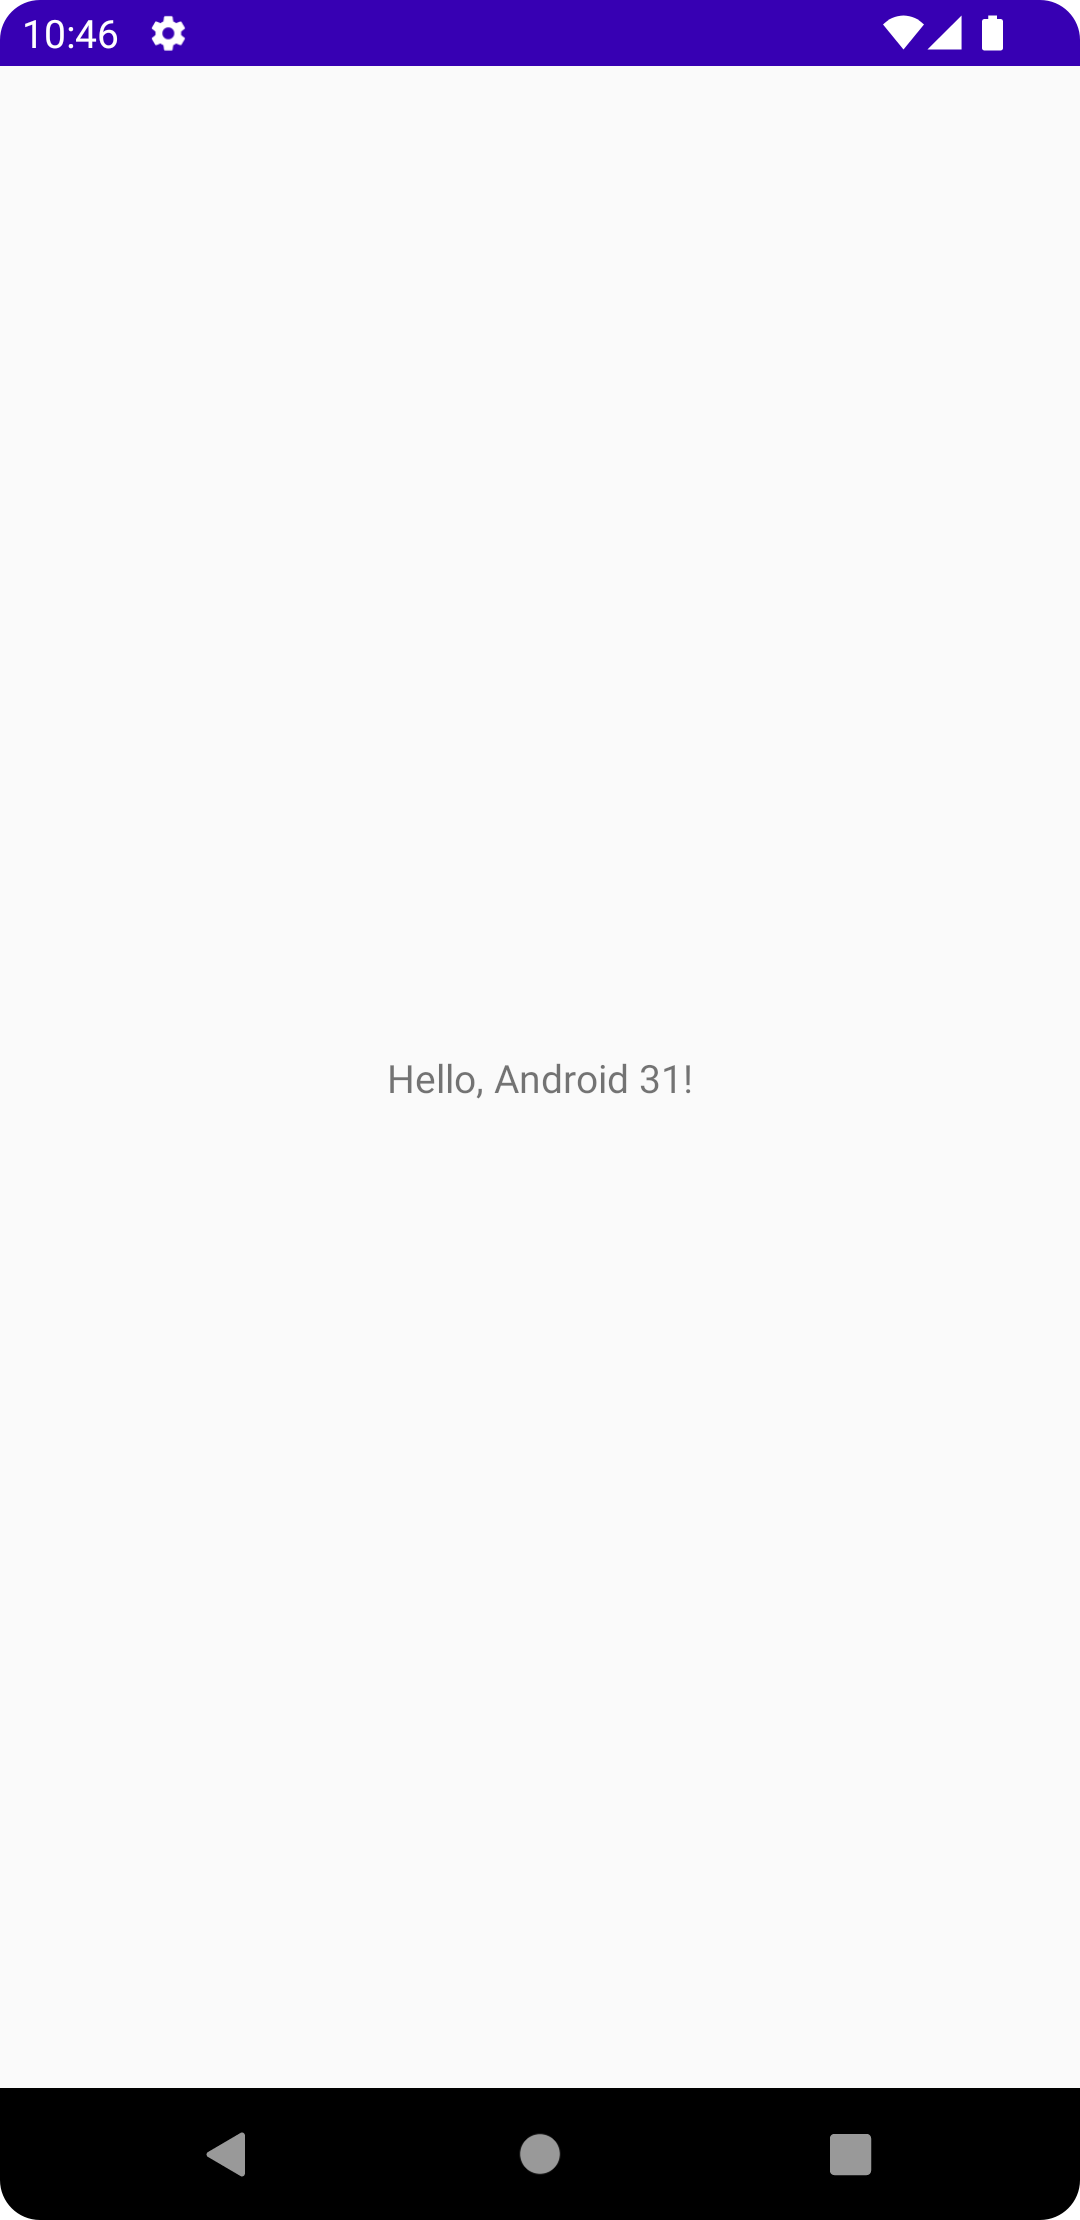
\includegraphics[width=0.37\textwidth]{img/kmm_example_android.png}
        \caption{Esempio expect/actual in esecuzione sulla piattaforma Android}
        \label{expect-actual-android}
    \end{figure}

    \begin{figure}[H]
        
\includegraphics[width=0.35\textwidth]{img/kmm_example_ios_dark.png}
        \caption{Esempio expect/actual in esecuzione sulla piattaforma iOS}
        \label{expect-actual-ios}
    \end{figure}
\end{multicols}

\subsubsection{KMM Gradle Plugins}
Gli strumenti di build automation permettono la gestione di tutti quei task riguardanti la compilazione del codice. Gradle rappresenta il tool di build automation ufficiale Android ed è possibile sviluppare delle estensioni, chiamate plugins, per aggiungere task custom allo strumento. E' proprio tramite questo meccanismo che KMM permette l'esecuzione dei task relativi allo sviluppo di applicazioni mobile multiplatform.

Il plugin Gradle KMM fornisce uno specifico DSL\footnote{Domain Specific Language} per definire e configurare i task necessari a compilare il codice condiviso per le relative piattaforme target\footnote{\href{https://kotlinlang.org/docs/multiplatform-dsl-reference.html}{https://kotlinlang.org/docs/multiplatform-dsl-reference.html}}. Alcune delle principali tipologie di task sono:

\begin{itemize}
    \item \textbf{Build} - tasks per build, compile, link
    \item \textbf{CocoaPods} - tasks per la gestione delle dipendenze Swift/Objective-C
    \item \textbf{Interop} - tasks relativi all'utilizzo del \textit{commonizer}\footnote{\href{https://github.com/JetBrains/kotlin/tree/master/native/commonizer}{https://github.com/JetBrains/kotlin/tree/master/native/commonizer}}
    \item \textbf{Verification tasks} - tasks per l'esecuzione dei test
\end{itemize}

Lo strumento di build automation Gradle e i relativi plugins utilizzati vengono configurati tramite specifici file locati insieme ai sorgenti del progetto. Il seguente codice\footnote{\href{https://github.com/paganellif/DevOps-per-applicazioni-mobile-un-caso-di-studio-industriale/blob/3-applicazioni-multipiattaforma/kmm-example/shared/build.gradle.kts}{https://github.com/paganellif/DevOps-per-applicazioni-mobile-un-caso-di-studio-industriale/blob/3-applicazioni-multipiattaforma/kmm-example/shared/build.gradle.kts}} mostra come è possibile configurare il modulo condiviso tramite l'apposito DSL. E' in questo file di configurazione che si definiscono le specifiche dipendenze e task per le piattaforme target:

\begin{listing}[H]
\inputminted{kotlin}{code/3-gradlekmm2}
\caption{Definizione utilizzo Plugin Gradle KMM nel file \textit{build.gradle.kts} del modulo condiviso (Kotlin).}
\end{listing}

\subsection{Fastlane}
Nonostante vi sia la necessità di utilizzare diversi strumenti di build automation per l'esecuzione dei task di sviluppo per le due differenti piattaforme Android e iOS, il processo di sviluppo e le fasi che lo compongono sono comuni, indipendentemente dalla piattaforma target. Come descritto nei capitoli precedenti, lo sviluppatore deve essere in grado non solo di eseguire task strettamente correlati alla fase di sviluppo ma anche di eseguire tutti quei task che riguardano il testing, la stabilizzazione e il rilascio di una applicazione.

Tra gli strumenti open-source dedicati allo sviluppo di applicazioni multipiattaforma uno dei più popolari è sicuramente Fastlane\footnote{\href{7https://github.com/fastlane/fastlane}{7https://github.com/fastlane/fastlane}}. Il punto di forza di questo tool è il supporto a tutte le fasi del processo di sviluppo di applicazioni mobile per entrambe le piattaforme Android e iOS mettendo lo sviluppatore nella condizione di poter operare su tutto il processo tramite un unico tool.

I task del delle varie fasi del processo definiscono il comportamento di Fastlane e devono essere descritti negli appositi file di configurazione Fastfile e Appfile utilizzando due concetti principali:

\begin{itemize}
    \item \textbf{Action} - Elaborazione pre-definita e configurabile tramite passaggio di parametri, rappresenta il task che deve essere eseguito.
    \item \textbf{Lane} - Insieme di action definito dall'utente per descrivere elaborazioni complesse, ovvero task composti da più sotto-task.
\end{itemize}

Il seguente codice\footnote{\href{https://github.com/paganellif/DevOps-per-applicazioni-mobile-un-caso-di-studio-industriale/blob/3-applicazioni-multipiattaforma/fastlane/fastlane/Fastfile}{https://github.com/paganellif/DevOps-per-applicazioni-mobile-un-caso-di-studio-industriale/blob/3-applicazioni-multipiattaforma/fastlane/fastlane/Fastfile}} rappresenta un esempio di lane Fastlane per il rilascio in versione beta di applicazioni iOS. Tale lane, chiamata \textit{beta}, è composta da quattro action rispettivamente per: (\textit{i}) inizializzare l'ambiente per connettersi ai servizi cloud Apple e scaricare tutto il necessario per la fase di firma del codice, (\textit{ii}) compilazione del codice Swift e creazione del pacchetto \textit{ipa} contenente l'applicazione iOS, (\textit{iii}) pubblicazione in versione beta su Testflight e (\textit{iv}) invio della notifica dell'avvenuta pubblicazione su un canale Slack dedicato.

\begin{listing}[H]
    \inputminted{ruby}{code/4-fastlane}
    \caption{Esempio di definizione di una lane Fastlane per il rilascio in versione beta di applicazioni iOS}
\end{listing}

\clearpage{\pagestyle{empty}\cleardoublepage}
\chapter{Caso di studio: applicazione MaggioliEbook}
\label{ch:casodistudio}
% !TeX root = ../main.tex

\section{Introduzione}
In questo capitolo vengono inizialmente descritte le motivazioni che hanno spinto l'azienda Maggioli S.p.A.\footnote{\href{https://www.maggioli.com/en-us}{https://www.maggioli.com/en-us}} a dedicare risorse per la ricerca e la sperimentazione nei campi delle applicazioni multipiattaforma e delle tecniche DevOps in ambito mobile.
Successivamente sono indicati i requisiti del caso di studio industriale individuato, 
il quale può essere suddiviso in due macroaree:

\begin{itemize}
    \item definizione del processo di sviluppo per applicazioni multipiattaforma tramite l'adozione della cultura DevOps,
    
    \item sviluppo di un'applicazione mobile multipiattaforma utilizzando il processo di sviluppo definito.
\end{itemize}

\section{Contesto aziendale}
Tra i core business dell'azienda Maggioli S.p.A. è rimasto centrale il ruolo dell'editoria,
ma col trascorrere degli anni e il mutare delle esigenze dei clienti, 
i quali sono principalmente pubblica amministrazione (PA) e professionisti privati, 
come avvocati, 
architetti, 
commercialisti ed ingegneri edili, 
si è verificata una transizione verso il mondo digitale.

I servizi digitali erogati per la consultazione delle pubblicazioni hanno superato considerevolmente il formato cartaceo,
il quale rimane comunque un metodo secondario di consultazione disponibile seppur in forma molto ridotta. 
Per l'editoria digitale esiste in Maggioli una business unit dedicata, 
chiamata \textit{Digital Media}, 
il cui ruolo principale consiste nella realizzazione e manutenzione dei siti Web Maggioli dedicati alla ricerca e visualizzazione delle pubblicazioni digitali. 
I seguenti sono soltanto alcuni dei siti gestiti dal team \textit{Digital Media}: 
Biblioteca Digitale\footnote{\href{https://bibliotecadigitale.maggioli.it/}{https://bibliotecadigitale.maggioli.it/}}, 
Appalti \& Contratti\footnote{\href{https://www.appaltiecontratti.it/}{https://www.appaltiecontratti.it/}} e Periodici\footnote{\href{https://www.periodicimaggioli.it/}{https://www.periodicimaggioli.it/}}. 
La necessità principale è dunque quella di fare innovazione tramite lo sviluppo di un'applicazione mobile in modo da fornire ai clienti Maggioli un nuovo metodo di accesso alle pubblicazioni che sia più accessibile e comodo.

\begin{figure}[H]
    \centering
    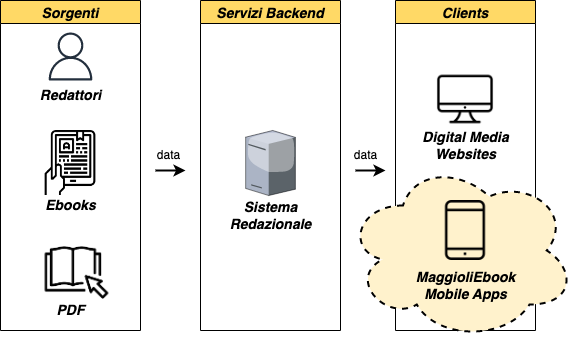
\includegraphics[width=0.75\textwidth]{img/contesto-aziendale.png}
    \caption{Schema del contesto aziendale in cui è collocato il caso di studio}
    \label{contesto-aziendale-fig}
\end{figure}

Le motivazioni che stanno alla base della scelta della cultura DevOps e delle applicazioni multipiattaforma per lo sviluppo di questo caso di studio sono comuni a qualsiasi tipologia d'azienda: 
come descritto nei capitoli \ref{ch:devops} e \ref{ch:app-multiplatform} è possibile ottimizzare il processo di sviluppo diminuendo le risorse impiegate e quindi i costi ma allo stesso tempo aumentando la qualità del software e la frequenza di rilascio,
i quali comportano una maggiore soddisfazione sia da parte dell'utente finale che da parte dell'azienda.

\section{Definizione processo di sviluppo}
Considerando l'intero contesto aziendale esistono degli standard, 
consolidati con l'esperienza maturata nello sviluppo software, 
che devono essere adottati sia per quanto riguarda il processo di sviluppo che la scelta degli strumenti necessari. 
L'obiettivo è riuscire a definire un modello di processo fortemente basato sugli standard aziendali ma adattato alle esigenze dello sviluppo di applicazioni mobile multipiattaforma e che possa essere introdotto nei team che si occupano di applicazioni mobile. 
I principali standard aziendali riguardanti gli strumenti e le tecnologie che devono essere adottati sono:

\begin{itemize}
    \item \textbf{GitLab}\footnote{\href{https://about.gitlab.com/}{https://about.gitlab.com/}} (\textit{DVCS/CI Server}) - Le funzionalità necessarie al versionamento del codice, alla collaborazione/pianificazione e all'automazione (Sezione \ref{devops-tools-sec}) sono tutte soddisfatte dalla piattaforma cloud GitLab con la quale è presente una sottoscrizione di piano di licenza aziendale.
    
    \item \textbf{SonarQube}\footnote{\href{https://www.sonarqube.org/}{https://www.sonarqube.org/}} (\textit{Vulnerability Management System}) - Questo servizio self-hosted è reso disponibile a tutti i team aziendali e permette di soddisfare gran parte dei task di Continuous Inspection. Grazie a SonarQube è possibile effettuare l'analisi statica del codice, validare il rispetto di determinate policy aziendali e visualizzare dashboard sullo stato delle scansioni.
    
    \item \textbf{Renovate}\footnote{\href{https://docs.renovatebot.com/}{https://docs.renovatebot.com/}} (\textit{Dependency Management}) - Strumento utilizzato per automatizzare la gestione delle dipendenze dei progetti. 
\end{itemize}

La pipeline standard a livello aziendale, 
base di partenza per la definizione della pipeline per applicazioni mobile multipiattaforma, 
rispetta a pieno tutte le considerazioni fatte nel capitolo \ref{ch:devops} per tutte le tecniche d'automazione indicate (fig. \ref{ci-inspection-pipeline}). 
Tramite l'adattamento delle fasi di integration, delivery e inspection di questa pipeline con le necessità dello sviluppo mobile indicate nei capitoli \ref{ch:sdlc} e \ref{ch:app-multiplatform} si ottengono i seguenti requisiti e dunque la pipeline obiettivo da realizzare.

\subsection{Requisiti}
\begin{itemize}
    \item \textbf{R1} - Continuous Integration
    \begin{itemize}
        \item \textbf{R1.1} - Stage di compilazione, testing e packaging con i relativi sotto-task per entrambe le piattaforme Android e iOS.
        
        \item \textbf{R1.2} - L'output dell'ultimo stage deve essere un pacchetto contenente l'applicazione da passare come artefatto alla fase successiva di delivery.
        
        \item \textbf{R1.3} - Utilizzo del sistema aziendale di gestione automatica delle dipendenze Renovate.
    \end{itemize}
    
    \item \textbf{R2} - Continuous Delivery
    \begin{itemize}
        \item \textbf{R2.1} - Stage di stabilizzazione suddivisi tra \textit{Alpha} e \textit{Beta} per il testing interno ed esterno tramite gli appositi servizi forniti da Google e Apple: Google Play Console per l'applicazione Android e Testflight per l'applicazione iOS.
        
        \item \textbf{R2.2} - L'applicazione soggetta a stabilizzazione è data in input dalla fase precedente di integrazione.
        
        \item \textbf{R2.3} - Stage di pubblicazione sui relativi marketplace Google Play Store o App Store. L'applicazione soggetta a pubblicazione deriva dalla terminazione con successo della fase di stabilizzazione e si trova già sui portali utilizzati.
    \end{itemize}
    
    \item \textbf{R3} - Continuous Inspection
    \begin{itemize}
        \item \textbf{R3.1} - Stage di analisi statica e analisi delle dipendenze per entrambe le piattaforme.
        
        \item \textbf{R3.2} - Utilizzo del sistema aziendale di gestione delle vulnerabilità centralizzato SonarQube.
    \end{itemize}
    
    \item \textbf{R4} - Tutto il sistema di automazione deve poter essere utilizzato da altri team di sviluppo all'interno dell'azienda.
\end{itemize}

\begin{figure}[H]
    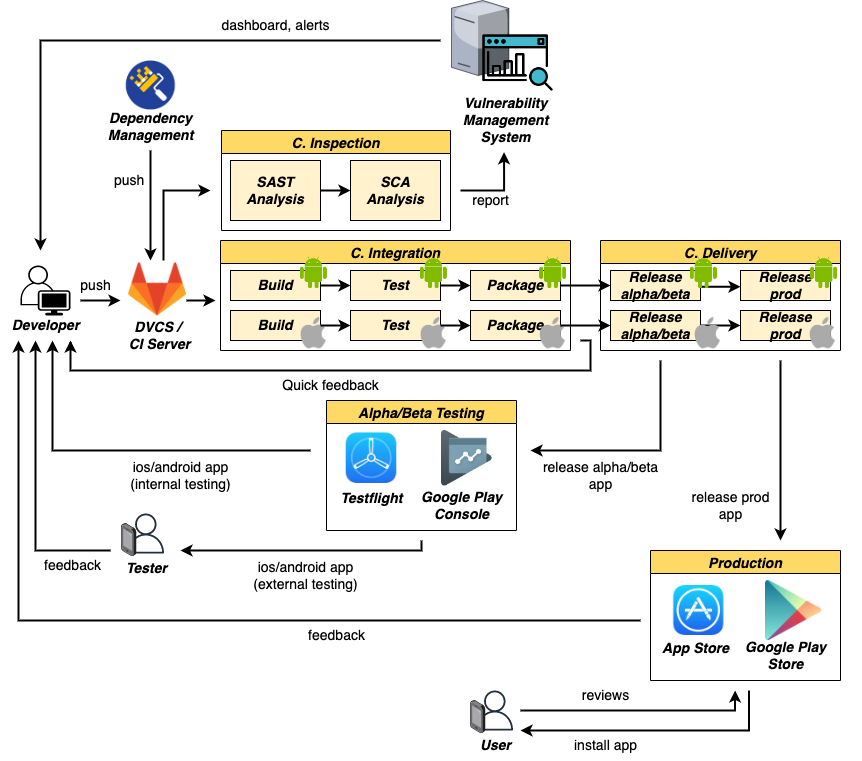
\includegraphics[width=1\textwidth]{img/full-cicd.png}
    \caption{Schema globale del processo di sviluppo automatizzato che si intende realizzare}
    \label{full-cicd}
\end{figure}

\section{Definizione applicazione}
Dato il contesto aziendale dell'editoria digitale in cui si colloca il caso di studio,
è possibile catalogare l'applicazione mobile da sviluppare come \textit{E-Reader}. 
Un e-book reader, 
chiamato anche e-book device o e-reader, 
è un dispositivo elettronico mobile progettato principalmente per la lettura di e-book e periodici digitali. 
Ogni dispositivo in grado di mostrare del testo su uno schermo potrebbe essere considerato un e-reader, 
ma i dispositivi progettati appositamente per questo compito hanno caratteristiche e funzionalità specifiche come l'ottimizzazione della portabilità, 
la leggibilità e la durata della batteria~\cite{shoba2014vocabulary}.

Per poter avere un valore aggiunto rispetto alle funzionalità già fornite dai siti Web sviluppati dal team \textit{Digital Media},
l'applicazione ``MaggioliEbook'' deve comportarsi come un vero e proprio e-reader, 
integrandosi ai servizi backend Maggioli per l'editoria digitale già esistenti. 
Data la complessità del dominio da modellare sono stati svolti degli incontri con figure interne esperte di dominio appartenenti ai team \textit{Ricerca e Sviluppo} e \textit{Digital Media}, 
al fine di definire (\textit{i}) terminologia, 
(\textit{ii}) casi d'uso e (\textit{iii}) requisiti.

\subsection{Terminologia e casi d'uso}
E' necessario che il team di sviluppo, 
composto da figure tecniche, 
e i committenti, 
i quali sono invece esperti interni di dominio, 
utilizzino lo stesso linguaggio per far si che le successive fasi del processo siano efficaci ed efficienti. 

Il concetto di \textit{Ubiquitous Language} definisce un vocabolario condiviso da entrambe le parti per la discussione del software~\cite{evans_domain-driven_2004} ed è stato adottato per la realizzazione del seguente glossario, 
il quale racchiude tutti i principali termini utilizzati negli incontri tra team di sviluppo ed esperti di dominio, 
suddivisi in \textit{entità} e \textit{casi d'uso}:

\subsubsection*{Entità}
\begin{table}[H]
\centering
    \begin{tabular}{|c|c|}
         \hline
         \textbf{Termine} & \textbf{Descrizione}\\
         \hline
         \textit{Reader} & \specialcell{Lettore di documenti in grado di visualizzarli ed \\interagire con essi.}\\
         \hline
         \textit{Documento} & Contenuto digitale pubblicato da Maggioli Editore.\\
         \hline
         \textit{Documento Statico} & Documento con una certa struttura definita (PDF).\\
         \hline
         \textit{Documento Fluido} & \specialcell{Documento senza struttura in grado di adattarsi al dispositivo\\ in cui viene aperto (EPUB).}\\
         \hline
         \textit{Libro} & \specialcell{Tipologia principale di documento fluido fruibile\\ tramite l'applicazione MaggioliEbook.}\\
         \hline
         \textit{Rivista} & \specialcell{Tipologia principale di documento statico fruibile\\ tramite l'applicazione MaggioliEbook.}\\
         \hline
         \textit{Bookmark} & Identifica una specifica pagina di un libro o di una rivista.\\
         \hline
         \textit{Progression} & \specialcell{Progresso di lettura di un libro o di una rivista,\\ calcolato in percentuale \\(numero di pagine lette sul totale del documento).}\\
         \hline
         \textit{Highlight} & \specialcell{Annotazione per una certa porzione testuale di \\documento. Può essere una evidenziazione, sottolineatura \\o annotazione testuale.}\\
         \hline
         \textit{Favorite} &  Documento preferito dall'utente.\\
         \hline
         \textit{User} & Utente con uno o più abbonamenti attivi.\\
         \hline
          \textit{Token} & \specialcell{Autentica e autorizza l'utente ad accedere ai vari documenti\\ per i quali esiste un abbonamento attivo.}\\
         \hline
    \end{tabular}
    \caption{Glossario dei termini (Entità)}
\end{table}

\newpage
\subsubsection*{Casi d'uso}
\begin{table}[H]
\centering
    \begin{tabular}{|c|c|}
         \hline
         \textbf{Termine} & \textbf{Descrizione}\\
         \hline
         \textit{Apertura Documento} & \specialcell{Richiesta di apertura in lettura di uno specifico\\ documento.}\\
         \hline
         \textit{Chiusura Documento} & Richiesta di chiusura del documento aperto in lettura.\\
         \hline
         \textit{Ricerca Documento} & Richiesta di ricerca documento tramite query testuale.\\
         \hline
         \specialcell{\textit{Lettura Metadati}\\\textit{Documento}} & Richiesta di lettura metadati documento.\\
         \hline
         \textit{Creazione Highlight} & Richiesta di creazione annotazioni.\\
         \hline
         \textit{Lettura Highlight} & Richiesta di lettura annotazioni.\\
         \hline
         \textit{Eliminazione Highlight} & Richiesta di eliminazione annotazioni.\\
         \hline
         \textit{Creazione Bookmark} & Richiesta di creazione segnalibri.\\
         \hline
         \textit{Lettura Bookmark} & Richiesta di lettura segnalibri.\\
         \hline
         \textit{Eliminazione Bookmark} & Richiesta di eliminazione segnalibri.\\
         \hline
         \textit{Creazione Progression} & \specialcell{Richiesta di salvataggio dell'\\avanzamento di lettura di un documento.}\\
         \hline
         \textit{Lettura Progression} &  \specialcell{Richiesta di lettura dell'\\avanzamento di lettura di un documento.}\\
         \hline
         \textit{Eliminazione Progression} &  \specialcell{Richiesta di eliminazione dell'\\avanzamento di lettura di un documento.}\\
         \hline
         \textit{Creazione Favorite} &  Richiesta di creazione preferiti.\\
         \hline
         \textit{Lettura Favorite} & Richiesta di lettura preferiti.\\
         \hline
         \textit{Eliminazione Favorite} & Richiesta di eliminazione preferiti.\\
         \hline
         \specialcell{\textit{Conversione}\\\textit{PDF2EPUB}} & \specialcell{Richiesta di conversione di un documento statico in\\ documento fluido (dal formato PDF al formato EPUB).}\\
         \hline
         \specialcell{\textit{Download Contenuto}\\\textit{Documenti}} & Scaricamento del contenuto dei documenti.\\
         \hline
         \specialcell{\textit{Download Copertina}\\\textit{Documenti}} & \specialcell{Scaricamento della immagine di copertina dei \\documenti.}\\
         \hline
         \textit{Login User} & Richiesta di login dell'utente (lettura token).\\
         \hline
         \textit{Logout User} & Richiesta di logout dell'utente (eliminazione token).\\
         \hline
         \specialcell{\textit{Controllo Login}\\\textit{User}} & \specialcell{Controllo di autenticazione dell'utente\\ già avvenuta (esistenza token).}\\
         \hline
         \specialcell{\textit{Lettura Account Utente}} & Richiesta informazioni utente (dati anagrafici e mail).\\
         \hline         
    \end{tabular}
    \caption{Glossario dei termini (Casi d'uso)}
\end{table}
\newpage

\begin{figure}[H]
\centering
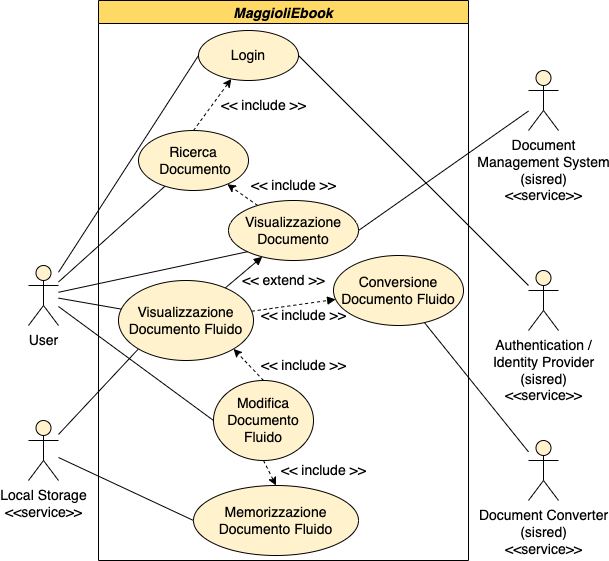
\includegraphics[width=1\textwidth]{img/casi-uso-uml.png}
\caption{UML - Diagramma dei casi d'uso: funzioni/servizi offerti dalla applicazione MaggioliEbook}
\end{figure}

\begin{figure}[H]
\centering
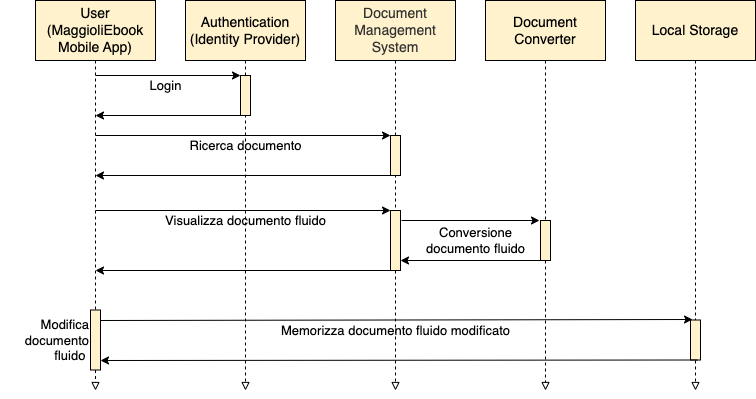
\includegraphics[width=1\textwidth]{img/caso-uso-sequenza-uml.png}
\caption{UML - Diagramma di sequenza: scenario di modifica di un nuovo documento "fluido"}
\end{figure}

\subsection{Requisiti}
\begin{itemize}
    \item \textbf{R1} - Visualizzazione documenti.
    \begin{itemize}
        \item \textbf{R1.1} - In modo fluido, mostrando il contenuto adattato al dispositivo in cui viene mostrato.
        
        \item \textbf{R1.2} - In modo statico, mostrando il contenuto con uno specifico layout indipendente dal dispositivo in cui viene mostrato.
    \end{itemize}
    
    \item \textbf{R2} - Modifica documenti fluidi (lato utente).
    \begin{itemize}
        \item \textbf{R2.1} - Aggiunta segnalibri, commenti, sottolineature, evidenziazioni, al contenuto fluido.
        
        \item \textbf{R2.2} - Memorizzazione segnalibri, commenti, sottolineature, evidenziazioni apportate al contenuto fluido.
    \end{itemize}
    
    \item \textbf{R3} - Gestione utente.
    \begin{itemize}
        \item \textbf{R3.1} - Login (autenticazione) utente.
        
        \item \textbf{R3.2} - Visualizzazione documenti a cui l'utente è abbonato.
    \end{itemize}
    
    \item \textbf{R4} - Ricerca documenti.
    
    \item \textbf{R5} - Conversione documenti da modo statico a modo fluido.
    
    \item \textbf{R6} - Modifica documenti in modo fluido (lato azienda).
    \begin{itemize}
        \item \textbf{R6.1} - Aggiunta elementi/contenuti al documento in modo fluido (hyperlink, quiz, video, immagini, ...).
        
        \item \textbf{R6.2} - Memorizzazione elementi/contenuti aggiunti al documento fluido (hyperlink, quiz, video, immagini, ...).
    \end{itemize}
\end{itemize}

\clearpage{\pagestyle{empty}\cleardoublepage}
\chapter{Automazione del processo di sviluppo}
\label{ch:cicd}
% !TeX root = ../main.tex

\section{Introduzione}
Nei precedenti capitoli sono stati introdotti i concetti alla base della cultura DevOps, del ciclo di vita del processo di sviluppo di applicazioni mobile e delle applicazioni multipiattaforma, arrivando a definire un caso di studio industriale. In questo capitolo viene descritto come è stato effettivamente realizzato il sistema per l'automazione del processo di sviluppo nel rispetto dei requisiti e delle specifiche indicate nel capitolo precedente.

In questa fase di realizzazione del sistema di automazione e di implementazione della pipeline viene considerato il progetto base\footnote{\href{https://github.com/paganellif/DevOps-per-applicazioni-mobile-un-caso-di-studio-industriale/tree/3-applicazioni-multipiattaforma/kmm-example}{https://github.com/paganellif/DevOps-per-applicazioni-mobile-un-caso-di-studio-industriale/tree/3-applicazioni-multipiattaforma/kmm-example}} fornito dal plugin KMM\footnote{\href{https://plugins.jetbrains.com/plugin/14936-kotlin-multiplatform-mobile}{https://plugins.jetbrains.com/plugin/14936-kotlin-multiplatform-mobile}} per Android Studio al fine di mantenere il focus sul processo in modo più agnostico possibile rispetto ad una specifica applicazione utilizzatrice come può essere MaggioliEbook, argomento trattato nel capitolo successivo.

\section{Self-Hosted MacOS GitLab Runner}
% runner macos: in azienda non esistono runner macos.. riprendere il problema del fatto che apple obbliga a usare macOS, indicare le possibili soluzioni (runner managed/self-hosted, ecc) e come ho configurato il runner self-hosted
% approfondire tipologie di runner executor in gitlab e perche ho usato l'executor shell
Come anticipato nel capitolo \ref{ch:app-multiplatform} tutta la toolchain per lo sviluppo iOS è disponibile solamente per il sistema operativo macOS, il che implica la necessità di un ambiente macOS anche per l'esecuzione della pipeline, almeno per tutti i task riguardanti l'applicazione iOS. Esistono diversi modi per realizzare un sistema di automazione compatibile con i vincoli imposti da Apple e possono essere suddivisi nelle seguenti categorie:

\begin{itemize}
    \item \textbf{Soluzione completa as-a-Service} - Il grande interesse per l'automazione e lo sviluppo di applicazioni iOS da parte delle aziende ha portato alla nascita di servizi cloud completamente dedicati a questo scopo come ad esempio \textit{Bitrise}\footnote{\href{https://www.bitrise.io/home}{https://www.bitrise.io/home}} e \textit{XCode Cloud}\footnote{\href{https://developer.apple.com/xcode-cloud/}{https://developer.apple.com/xcode-cloud/}}.
    \item \textbf{Runner macOS managed} - Come anticipato nel capitolo \ref{ch:devops} un runner, ovvero il componente che esegue effettivamente i task della nostra pipeline, può essere \textit{managed} o \textit{self-hosted}. Nel caso di un runner managed con sistema operativo macOS si evita lo sforzo di configurare e mantenere un componente importante del sistema di automazione ma si hanno costi elevati: solitamente al consumo di risorse di questa tipologia di runner è applicato un fattore moltiplicativo poco sostenibile in termini di costi. Alcuni esempi di piattaforme con questo modello di business per i runner managed sono GitHub Action\footnote{\href{https://docs.github.com/en/billing/managing-billing-for-github-actions/about-billing-for-github-actions\#minute-multipliers}{https://docs.github.com/en/billing/managing-billing-for-github-actions/about-billing-for-github-actions\#minute-multipliers}} e GitLab CI\footnote{\href{https://docs.gitlab.com/ee/ci/pipelines/cicd\_minutes.html\#additional-costs-on-gitlab-saas}{https://docs.gitlab.com/ee/ci/pipelines/cicd\_minutes.html\#additional-costs-on-gitlab-saas}}.
    \item \textbf{Runner macOS self-hosted} - L'altra tipologia di runner consiste nella installazione del componente su una macchina con sistema operativo macOS che deve essere configurata e mantenuta dall'utilizzatore. In questo caso è possibile utilizzare macchine virtuali as-a-Service, come quelle fornite da AWS\footnote{\href{https://aws.amazon.com/ec2/instance-types/mac/}{https://aws.amazon.com/ec2/instance-types/mac/}} (Amazon Web Services), oppure hardware fisico Apple per installare ed eseguire il runner.
\end{itemize}

Data la disponibilità di tutta la toolchain Android per macOS e il costo nullo in caso di runner self-hosted, è stata scelta quest'ultima tipologia per l'esecuzione dell'intera pipeline.

L'installazione e la configurazione di un runner di questa tipologia può essere più o meno complicata in base alle funzionalità necessarie per il sistema di automazione. Nel caso specifico del caso di studio di questo progetto l'unica funzionalità richiesta da configurare è la cache condivisa al fine di abilitare la concorrenza tra più processi e ottimizzare l'esecuzione della pipeline.

I seguenti comandi bash\footnote{\href{https://github.com/paganellif/DevOps-per-applicazioni-mobile-un-caso-di-studio-industriale/blob/5-automazione-del-processo-di-sviluppo/setup-gitlab-macos-runner.sh}{https://github.com/paganellif/DevOps-per-applicazioni-mobile-un-caso-di-studio-industriale/blob/5-automazione-del-processo-di-sviluppo/setup-gitlab-macos-runner.sh}} mostrano la procedura di installazione di un runner GitLab macOS self-hosted su una macchina fisica Apple:
\begin{listing}[H]
    \inputminted{bash}{code/macos-runner-setup.sh}
    \caption{Comandi bash per l'installazione, la configurazione e l'avvio di un runner macOS self-hosted}
\end{listing}

Il seguente codice\footnote{\href{https://github.com/paganellif/DevOps-per-applicazioni-mobile-un-caso-di-studio-industriale/blob/5-automazione-del-processo-di-sviluppo/config.toml}{https://github.com/paganellif/DevOps-per-applicazioni-mobile-un-caso-di-studio-industriale/blob/5-automazione-del-processo-di-sviluppo/config.toml}} mostra il file di configurazione del runner, generato in seguito alla procedura sopra indicata:

\begin{listing}[H]
    \inputminted{toml}{code/macos-runner-config.toml}
    \caption{File di configurazione (\textit{config.toml}) generato al momento della installazione del runner}
\end{listing}

\section{Modello di branching}
L’utilizzo di un adeguato flusso di lavoro è fondamentale per definire una efficiente automazione CI/CD. Con branching si intende l’utilizzo di uno o più flussi principali dai quali divergono altri flussi per svolgere determinati lavori per poi convergere al loro termine: in base alle modalità di apertura e chiusura di questi flussi si definiscono diversi modelli di branching.

Il modello che si intende utilizzare (fig. \ref{branching}) è basato sul modello di branching GitFlow\footnote{\href{https://www.atlassian.com/it/git/tutorials/comparing-workflows/gitflow-workflow}{https://www.atlassian.com/it/git/tutorials/comparing-workflows/gitflow-workflow}} e prevede tre branch principali:

\begin{itemize}
    \item \textbf{dev} - Flusso principale di sviluppo. Ogni modifica apportata a questo branch corrisponde al rilascio di una nuova versione \textit{alpha} per la validazione interna. E' da questo branch che vengono aperti e chiusi nuovi branch, sia per lo sviluppo di nuove funzionalità (\textit{feature}) che per la risoluzione di bug/patch (\textit{fix}).

    \begin{figure}[H]
        \centering
        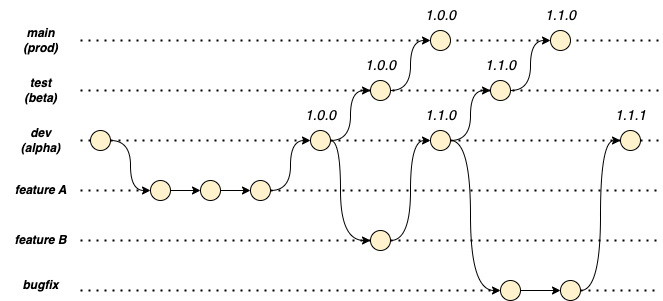
\includegraphics[width=0.65\textwidth]{img/branching-model.png}
        \caption{Esempio di flusso di sviluppo adottando il modello di branching indicato}
        \label{branching}
    \end{figure}
    
    \item \textbf{test} - Branch modificato solamente tramite merge di modifiche provenienti dal branch \textit{dev} con lo scopo di rilasciare una nuova versione \textit{beta} per la validazione esterna.
    \item \textbf{main} - Branch modificato solamente tramite merge di modifiche provenienti dal branch \textit{test} con lo scopo di rilasciare una nuova versione in produzione (\textit{prod}).
\end{itemize}

Grazie ai meccanismi di automazione a supporto della CI/CD fornite dal CI Server si definiscono specifiche regole di attivazione, chiamate \textit{trigger rules}, che permettono di indicare quando uno specifico job deve essere eseguito. Queste regole si basano su eventi che si verificano sul sistema di versionamento come ad esempio commit, tag e merge request. Tramite questa funzionalità è possibile dunque discriminare quali file sono stati modificati e su quale branch per eseguire le operazioni associate come descritto sopra.

\begin{figure}[H]
    \centering
    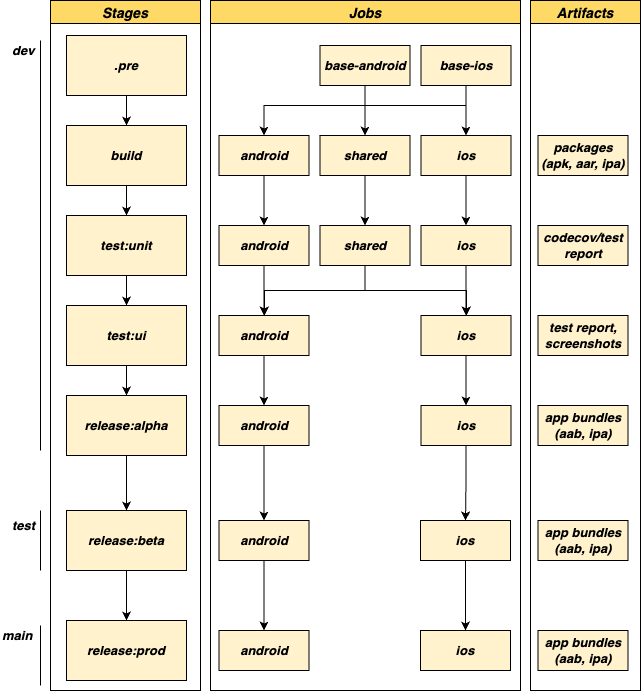
\includegraphics[width=0.85\textwidth]{img/cicd-branch-jobs.png}
    \caption{Stage, job e artefatti associati agli eventi sui branch che compongono l'intera pipeline}
\end{figure}

\section{Templating}
% strumenti utilizzati per favorire il riuso della cicd realizzata

\section{Continuous Integration}
\subsection{Pre}
Molti dei passi che compongono una pipeline utilizzano tipicamente gli stessi tools e le stesse configurazioni per svolgere task diversi. Ad esempio la compilazione del codice e l'esecuzione degli unit test per una applicazione Java utilizzano in entrambi i casi la stessa JDK\footnote{Java Development Kit}, lo stesso tool di build automation e devono essere scaricate le stesse dipendenze di progetto dal package manager di riferimento.

Utilizzando meccanismi di caching e passaggio di artefatti tra i vari job è possibile eseguire tutti quei task di configurazione una sola volta all'inizio della pipeline risparmiando tempo e risorse in tutte le fasi successive.

Nel caso della pipeline progettata per lo sviluppo di applicazioni multipiattaforma con KMM è necessario eseguire i seguenti task di configurazione iniziale:
\begin{itemize}
    \item Configurazione dell'ambiente per lo sviluppo Kotlin tramite l'installazione e il caching degli SDK e del sotto-compilatore \textit{Kotlin/Native}\footnote{\href{https://kotlinlang.org/docs/native-improving-compilation-time.html\#general-recommendations}{https://kotlinlang.org/docs/native-improving-compilation-time.html\#general-recommendations}} per lo sviluppo multipiattaforma.
    \item Configurazione dell'ambiente per lo sviluppo Android tramite l'installazione del SDK Android target e dei vari tools necessari tramite \textit{sdkmanager}\footnote{\href{https://developer.android.com/studio/command-line/sdkmanager}{https://developer.android.com/studio/command-line/sdkmanager}}.
    \item Configurazione dell'ambiente per lo sviluppo iOS tramite impostazione di XCode e CLI Developer Tools.
    \item Installazione e caching di tutte le dipendenze dei vari moduli.
    \item Configurazione delle chiavi per l'autenticazione ai servizi cloud forniti da Google e Apple.
\end{itemize}

Il seguente codice\footnote{\href{https://github.com/paganellif/DevOps-per-applicazioni-mobile-un-caso-di-studio-industriale/blob/5-automazione-del-processo-di-sviluppo/kmm-templates/kmm-base.yml}{https://github.com/paganellif/DevOps-per-applicazioni-mobile-un-caso-di-studio-industriale/blob/5-automazione-del-processo-di-sviluppo/kmm-templates/kmm-base.yml}} mostra il job di pre-configurazione per tutti i job successivi riguardanti la piattaforma Android:

\begin{listing}[H]
    \inputminted{yaml}{code/pre-android-job.yaml}
    \caption{Job di pre-configurazione Android}
\end{listing}

\subsection{Build e Packaging}
Tipicamente la fase di integrazione continua inizia con la verifica della corretta compilazione del codice sorgente. La compilazione rappresenta un vincolo essenziale per tutte le successive fasi e per questo è definita come fase bloccante: in caso di compilazione fallita la pipeline termina senza procedere con le fasi successive definite.

Nel caso dello sviluppo di applicazioni mobile, per lo stage iniziale di build la pratica più diffusa è quella di validare sia la compilazione del codice che la pacchettizzazione della applicazione nei formati richiesti dalle piattaforme target. Dato il funzionamento di una applicazione KMM (Capitolo \ref{ch:app-multiplatform}) è necessario compilare il codice del modulo condiviso \textit{shared} e quello specifico delle piattaforme Android e iOS e impacchettarlo negli artefatti che verranno passati in input alla fase di delivery, rispettivamente aar\footnote{Android Library}, aab e ipa.

Il seguente codice\footnote{\href{https://github.com/paganellif/DevOps-per-applicazioni-mobile-un-caso-di-studio-industriale/blob/5-automazione-del-processo-di-sviluppo/kmm-templates/kmm-build.yml}{https://github.com/paganellif/DevOps-per-applicazioni-mobile-un-caso-di-studio-industriale/blob/5-automazione-del-processo-di-sviluppo/kmm-templates/kmm-build.yml}} mostra il template che definisce il job base di compilazione e pacchettizzazione della applicazione Android tramite l'utilizzo combinato di fastlane e gradle:
\begin{listing}[H]
    \inputminted{yaml}{code/build-job.yaml}
    \caption{Pipeline job dedicato alla compilazione e pacchettizzazione della applicazione Android}
\end{listing}

\subsection{Testing}

\subsection{Dependency Management}

\section{Continuous Delivery}

\subsection{Alpha/Beta Release}

\section{Continuous Inspection}
% progettazione e implementazione analisi


\clearpage{\pagestyle{empty}\cleardoublepage}
\chapter{Sviluppo applicazione MaggioliEbook}
\label{ch:maggioliebook}
% !TeX root = ../main.tex

\section{Introduzione}

\section{Progettazione}
% progettazione app con mentalità multiplatform

\section{Implementazione modulo condiviso}
% implementazione modulo shared

\section{Implementazione Android}
% implementazione app android

\section{Implementazione iOS}
% implementazione app iOS

\clearpage{\pagestyle{empty}\cleardoublepage}
\chapter{Risultati raggiunti}
\label{ch:risultati}
% !TeX root = ../main.tex

\section{Introduzione}
In questo capitolo vengono mostrati i risultati ottenuti dalla realizzazione della applicazione multipiattaforma MaggioliEbook adottando il processo di sviluppo descritto nel capitolo \ref{ch:cicd}.

Vengono inizialmente considerati i requisiti definiti nel capitolo \ref{ch:casodistudio} e paragonati con quanto realizzato. Successivamente sono indicate alcune statistiche e metriche, raccolte principalmente tramite la piattaforma GitLab adottata, al fine di creare un primo modello di confronto per i lavori futuri che saranno svolti in azienda sulle tematiche principali di questo caso di studio industriale.

\section{Riuso}
I template che definiscono gli stage e i relativi job del processo di sviluppo progettato sono stati versionati e organizzati in un apposito repository, come descritto in modo dettagliato nel capitolo \ref{ch:cicd}.

Questa soluzione non solo permette il riuso dell'intera pipeline o di solamente una sua parte, ma abilita anche un processo di lavoro collaborativo fra tutti i possibili utilizzatori per la modifica del processo. Ogni sviluppatore all'interno della azienda è infatti in grado di accedere al repository dei template, visionare i file YAML che definiscono la pipeline e aprire merge request per richiedere la modifica o l'aggiunta di funzionalità necessarie al processo di sviluppo automatizzato. A tal proposito è stato scelto un team di sviluppo all'interno dell'azienda che si occupa di applicazioni mobile per svolgere un primo esperimento di integrazione nel proprio processo di sviluppo, già consolidato su tecnologie puramente native e senza alcun sistema di automazione.

\section{Stabilizzazione e rilascio}
La fase di stabilizzazione e rilascio di entrambe le versioni di applicazione sviluppate tramite Kotlin Multiplatform Mobile sono state realizzate rispettando tutti i vincoli definiti nel capitolo \ref{ch:casodistudio}. Durante il processo di sviluppo del caso di studio è stato infatti possibile rilasciare automaticamente applicazioni, sia Android che iOS, sfruttando la pipeline realizzata. In entrambi i casi sono stati definiti gruppi di tester composti sia dalle figure aziendali esperte di dominio che dai Professori relatori di questa tesi:

\begin{figure}[H]
    \centering
    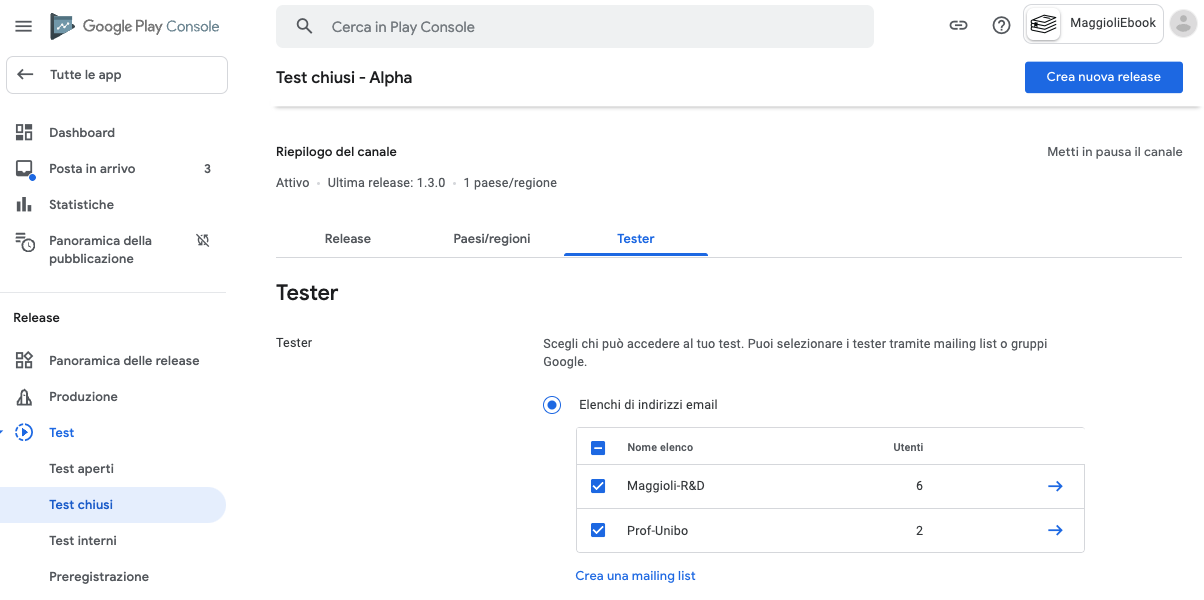
\includegraphics[width=1\textwidth]{img/google-play-console-maggioliebook.png}
    \caption{Schermata Google Play Console per la fase di stabilizzazione della applicazione Android}
    \label{google-play-console-maggioliebook}
\end{figure}

\begin{figure}[H]
    \centering
    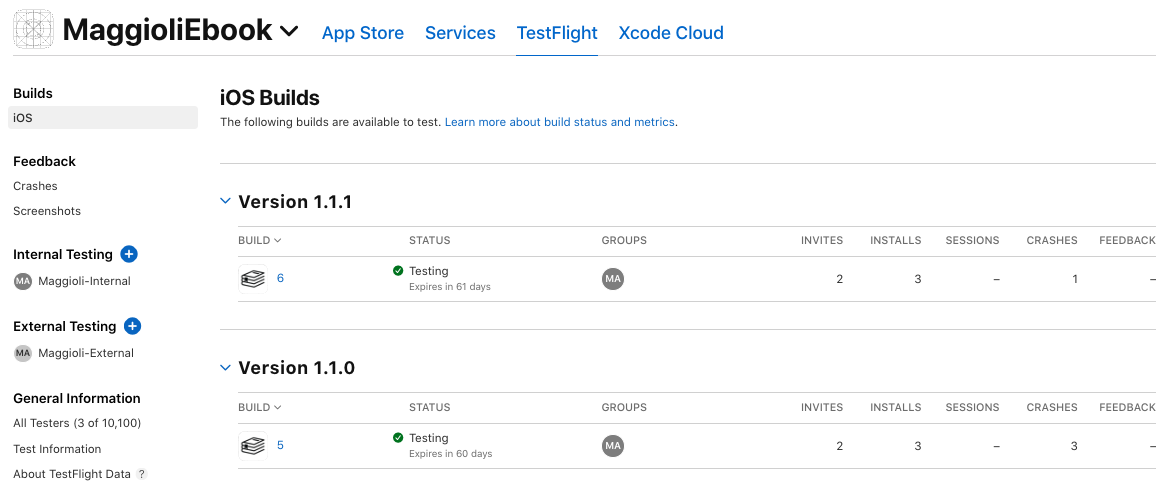
\includegraphics[width=1\textwidth]{img/app-store-connect-maggioliebook.png}
    \caption{Schermata App Store Connect per la fase di stabilizzazione della applicazione iOS}
    \label{app-store-connect-maggioliebook}
\end{figure}

Tutti i tester appartenenti ai gruppi configurati come nelle schermate precedenti sono poi stati in grado di installare con successo l'applicazione sul proprio dispositivo:

\begin{figure}[H]
    \centering
    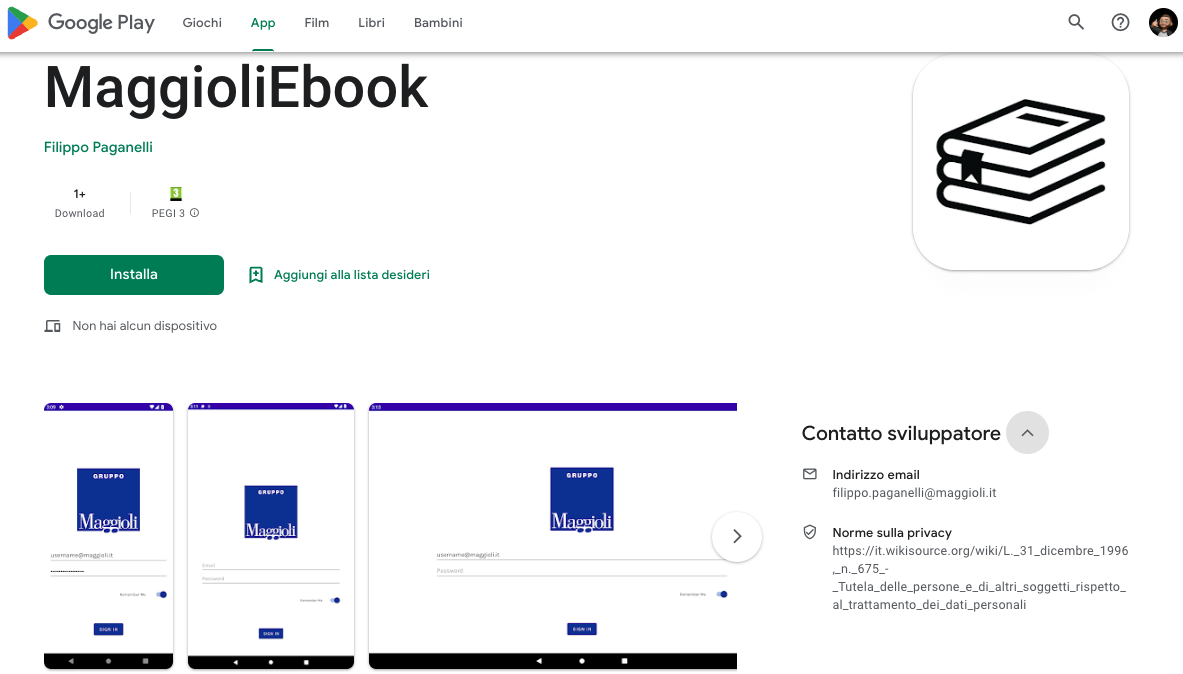
\includegraphics[width=1\textwidth]{img/google-play-store-maggioliebook.png}
    \caption{Schermata Google Play Store per la fase di stabilizzazione della applicazione Android}
    \label{google-play-store-maggioliebook}
\end{figure}

\begin{figure}[H]
    \centering
    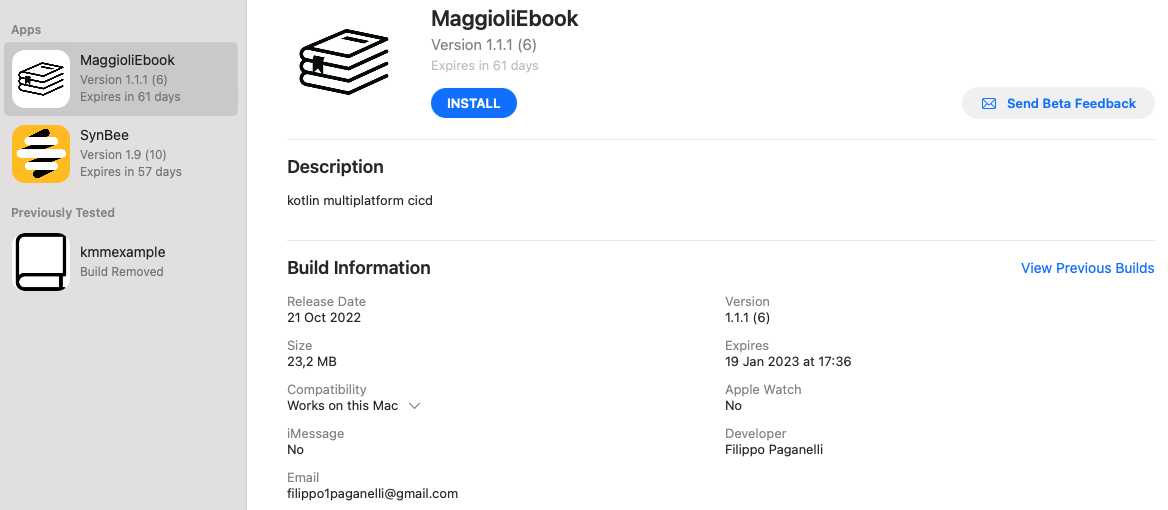
\includegraphics[width=1\textwidth]{img/testflight-maggioliebook.png}
    \caption{Schermata Testflight per la fase di stabilizzazione della applicazione iOS}
    \label{testflight-maggioliebook}
\end{figure}

Un ciclo di stabilizzazione \textit{alpha}-\textit{beta} risulta nell'esecuzione di due pipeline attivate rispettivamente con (\textit{i}) la modifica sul branch \textit{dev} del codice della applicazione e (\textit{ii}) il merge del branch \textit{dev} sul branch \textit{test}. Le seguenti schermate, catturate dalla piattaforma GitLab utilizzata come sistema di versionamento e automazione, mostrano l'esecuzione di un esempio di queste due pipeline nel caso della sola applicazione Android:

\begin{figure}[H]
\centering
    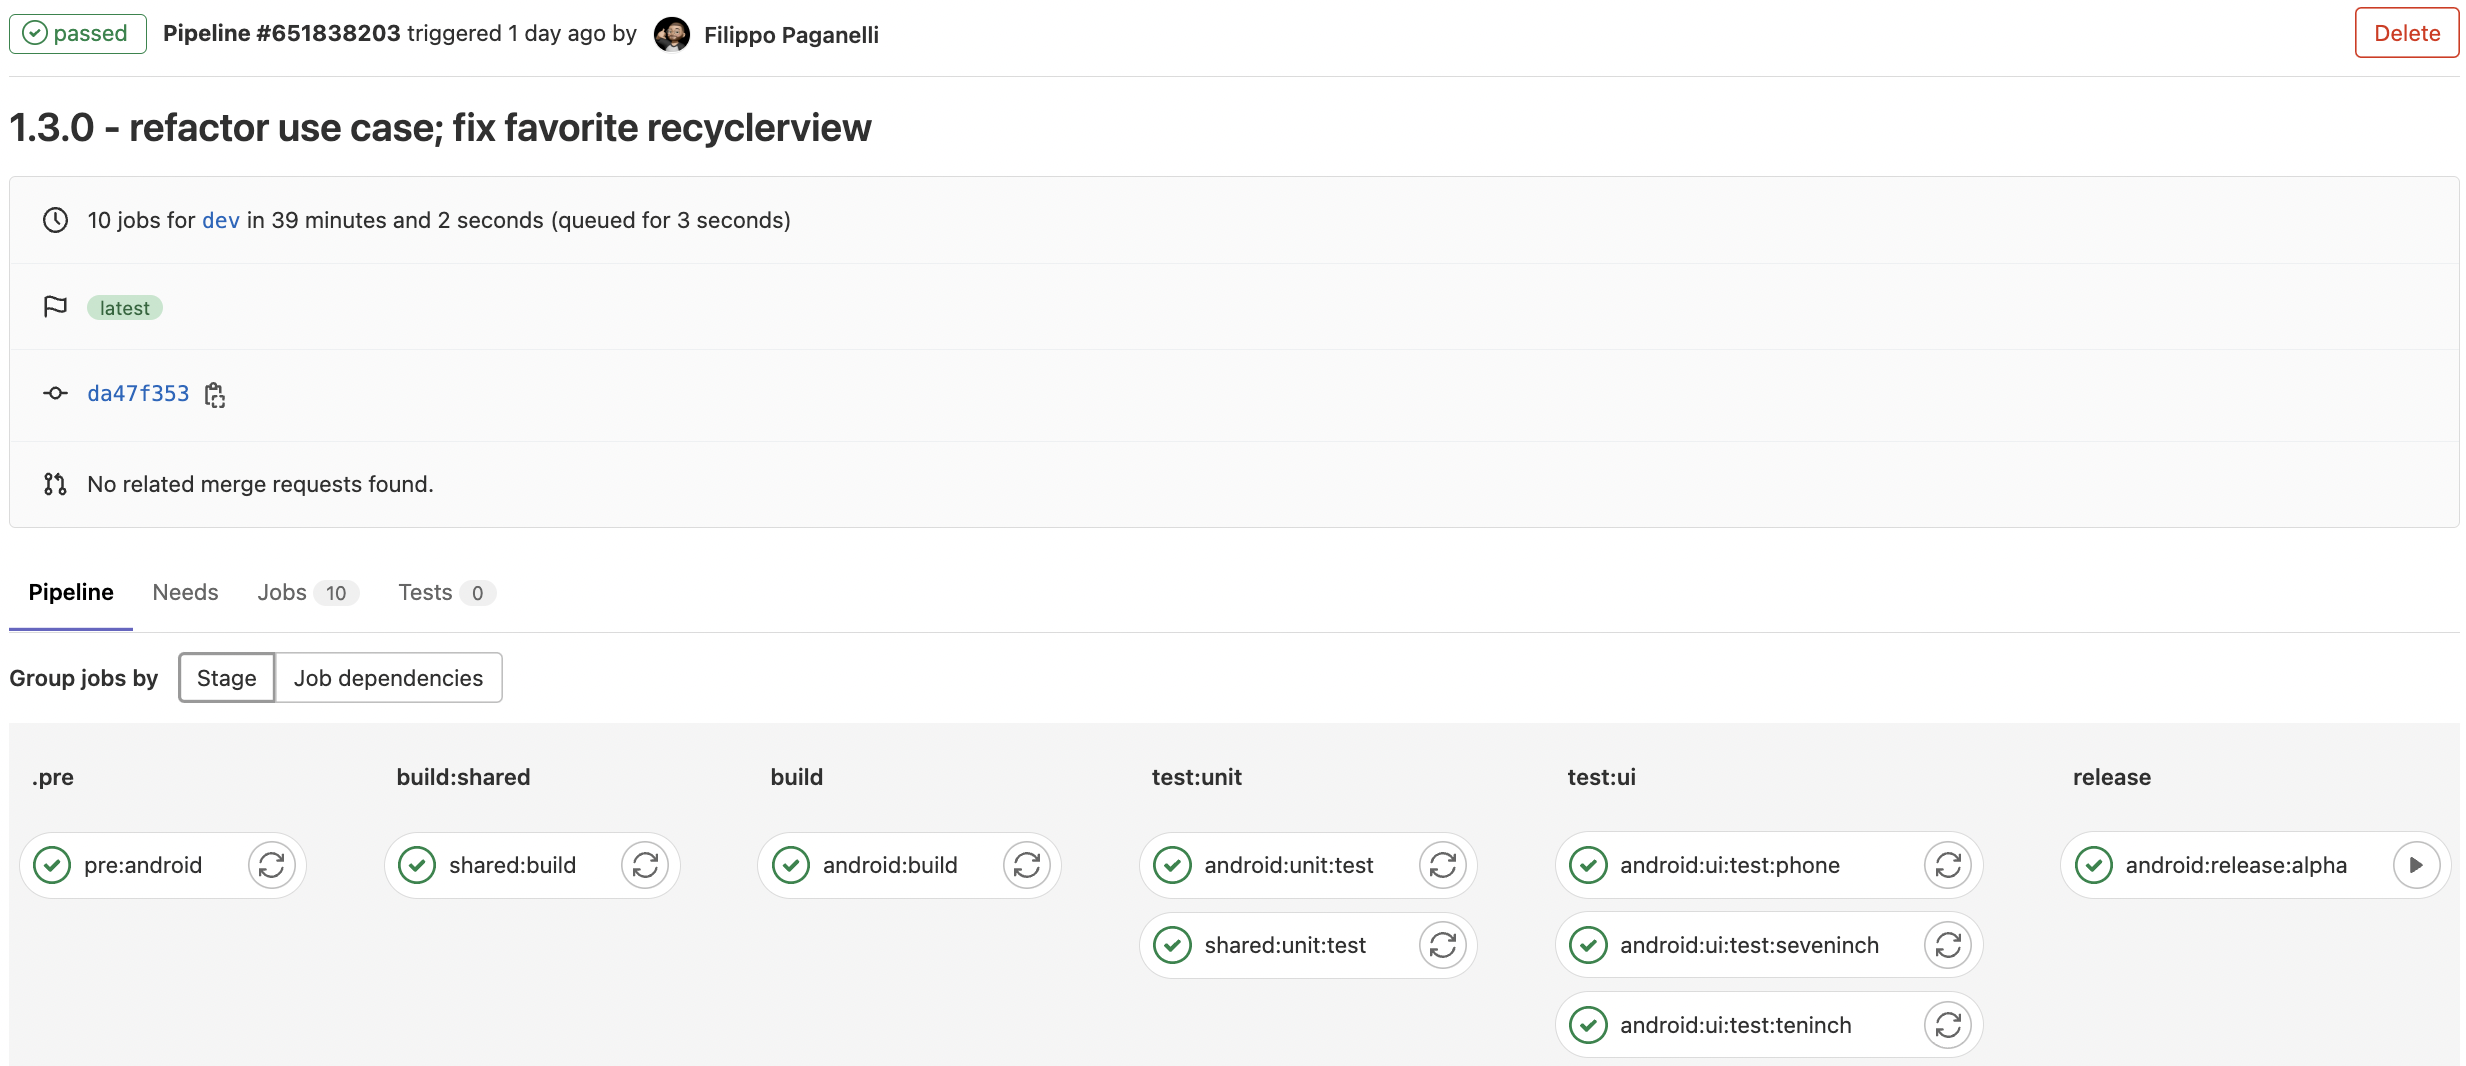
\includegraphics[width=1\textwidth]{img/gitlab-pipeline-android-alpha.png}
    \caption{Schermata GitLab di esecuzione della pipeline completa per il rilascio della applicazione Android in versione \textit{alpha}}
    \label{gitlab-pipeline-android-alpha}
\end{figure}

\begin{figure}[H]
\centering
    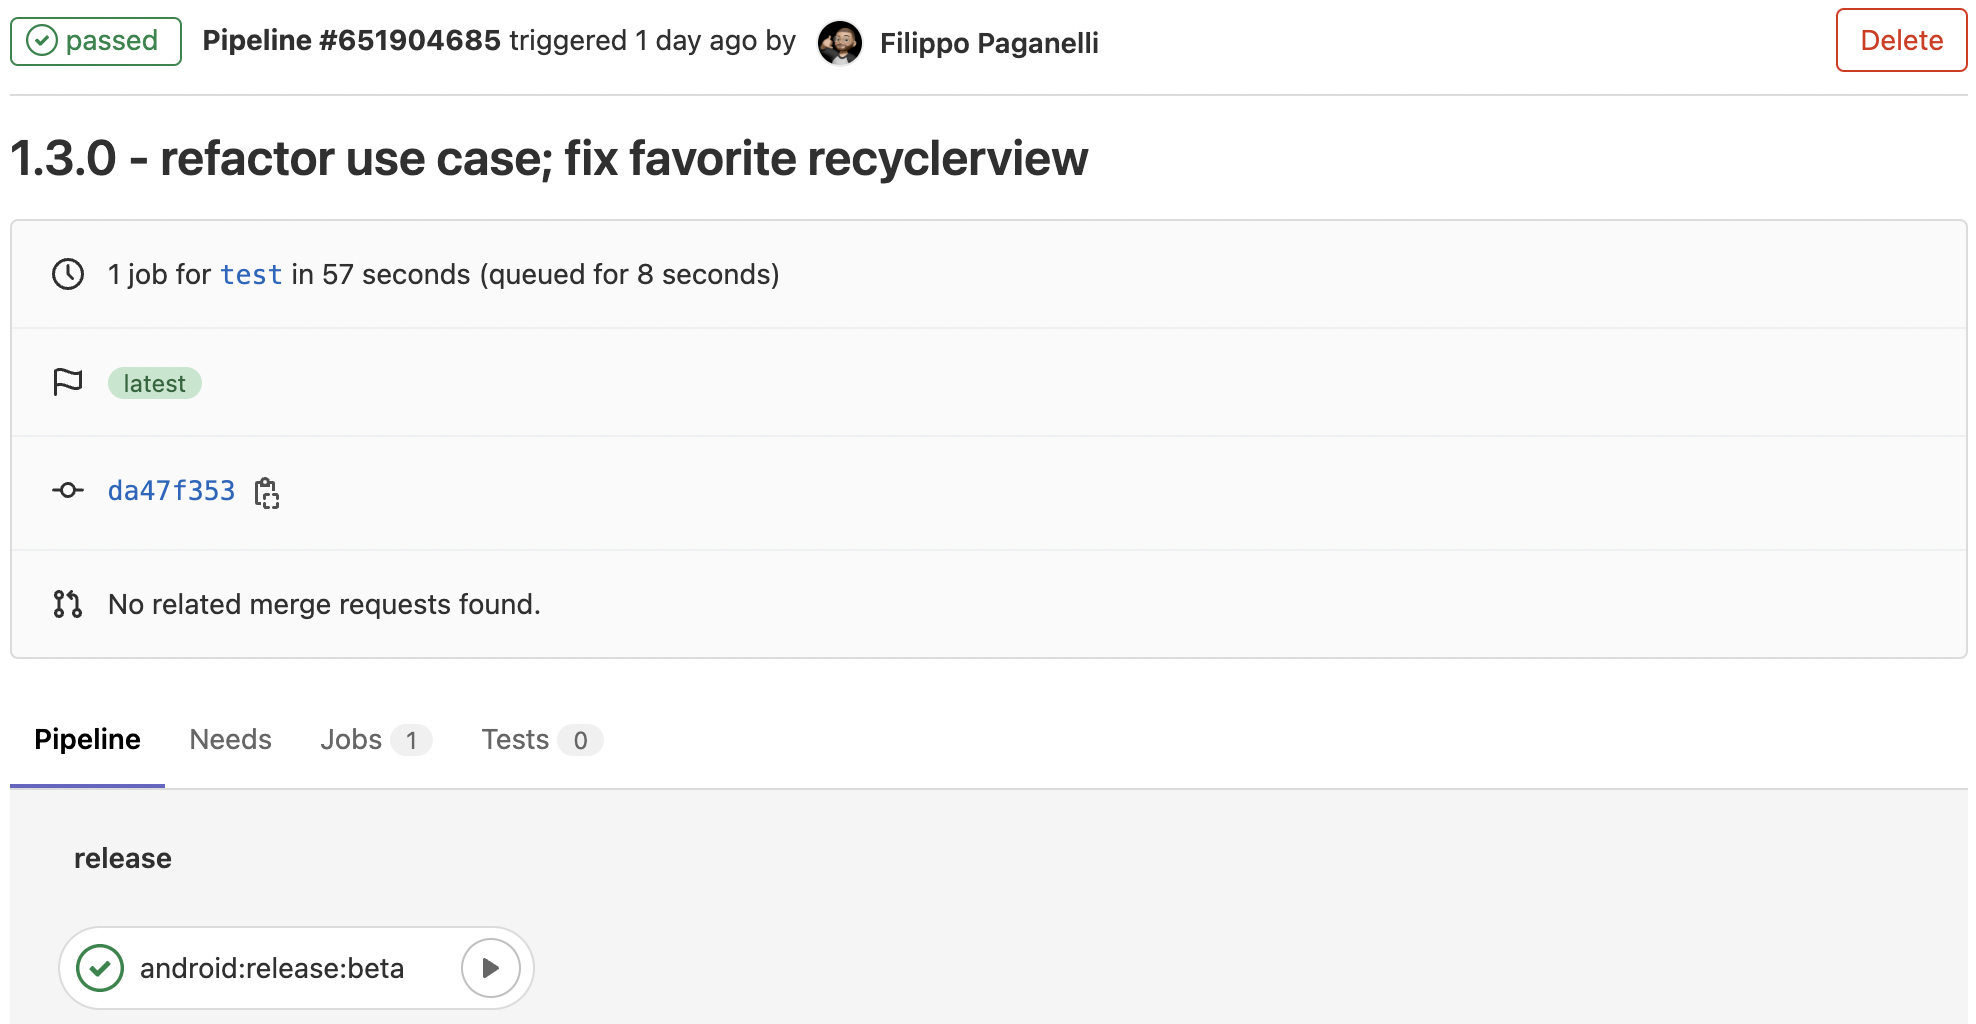
\includegraphics[width=1\textwidth]{img/gitlab-pipeline-android-beta.png}
    \caption{Schermata GitLab di esecuzione della pipeline completa per la promozione da versione \textit{alpha} a versione \textit{beta} della applicazione Android}
    \label{gitlab-pipeline-android-beta}
\end{figure}

\section{Analisi del codice}
% efficacia della pipeline di analisi

\section{Statistiche}
% qualche misurazione delle tempistiche di esecuzione delle pipeline nei vari casi (android, ios, ios+android e rilascio, analisi, ...)
% non ho parametri per fare il confronto rispetto a prima, la app sviluppata è nuova e altri team non hanno cicd app mobile

\section{Lavori futuri}
% cosa ho intenzione di fare dopo, continuazione del lavoro in azienda
\begin{itemize}
        \item Studio, ricerca e sperimentazione per la fase di monitoring, sia della applicazione che dell'utente.
        \item Utilizzo del meccanismo \textit{Remote Configuration}\footnote{\url{https://firebase.google.com/docs/remote-config}} per modificare aspetti della applicazione in modo dinamico senza dover rilasciare nuove versioni. Un esempio tipico è la migrazione dei database: grazie al meccanismo di remote configuration è possibile settare da remoto il \textit{jdbc}\footnote{Java DataBase Connectivity} url che permette di connettersi al database senza dover rilasciare una nuova versione della applicazione con il valore cablato nel codice.
        \item Valutazione di alternative all'hardware Apple fisico. Come indicato nel capitolo \ref{ch:cicd} alcune possibilità individuate sono: (\textit{i}) runner gestiti con sistema operativo MacOS (disponibili su diverse piattaforme come GitLab\footnote{\url{https://docs.gitlab.com/ee/ci/runners/saas/macos_saas_runner.html}}, GitHub\footnote{\url{https://docs.github.com/en/actions/using-github-hosted-runners/about-github-hosted-runners}} e CircleCI\footnote{\url{https://circleci.com/docs/using-macos}}), (\textit{ii}) virtual machine as-a-Service con sistema operativo MacOS (disponibili tra i servizi cloud Amazon\footnote{\url{https://aws.amazon.com/ec2/instance-types/mac/}}) e (\textit{iii}) immagine Docker MacOS\footnote{\url{https://github.com/sickcodes/Docker-OSX}}.
        \item Separazione dei moduli sviluppati in questo caso di studio in modo da avere più repository separati invece che la soluzione monorepo adottata. Distribuzione della logica applicativa sotto forma di libreria kmm e valutazione dei pro e contro di questa soluzione.
        \item Valutazione soluzioni complete as-a-Service. Ad esempio \textit{Bitrise}\footnote{\url{https://www.bitrise.io/}} o XCode Cloud\footnote{\url{https://developer.apple.com/documentation/xcode/xcode-cloud}} (solamente per la parte Apple).
        \item Sperimentazione tecniche CI/CD con tecnologie cross-platform come \textit{Ionic}\footnote{\url{https://ionicframework.com/}}, \textit{Flutter}\footnote{\url{https://flutter.dev/}} o \textit{React Native}\footnote{\url{https://reactnative.dev/}} e stesso caso d'uso (applicazione PoC MaggioliEbook) in modo da avere dei parametri di riferimento e confronto.
\end{itemize}

\clearpage{\pagestyle{empty}\cleardoublepage}
\chapter{Conclusioni}
\label{ch:conclusioni}
% !TeX root = ../main.tex

L'output finale di questa tesi dimostra che è stato possibile adottare le pratiche e gli strumenti abilitanti la cultura DevOps per il processo di sviluppo di applicazioni mobile multipiattaforma. Per poter ottenere un sistema di automazione in grado di compilare, testare, impacchettare e rilasciare una applicazione, sia in versione Android che in versione iOS, in circa 28 minuti in media come descritto nei risultati raggiunti (capitolo \ref{ch:risultati}) è stata necessaria una prima fase di analisi approfondita sulla cultura DevOps, sul ciclo di sviluppo delle applicazioni mobile e sui framework multipiattaforma. 

Successivamente è stato individuato un caso di studio per dimostrare l'efficacia della cultura DevOps applicata allo sviluppo mobile multipiattaforma in un contesto industriale. In questa fase sono stati raccolti i requisiti e i vincoli aziendali sia per il processo di sviluppo che per l'applicazione da realizzare in modo da adeguarli a quanto appreso dalla prima fase di studio e definire gli obiettivi reali.




%Per poter misurare con precisione i vantaggi derivanti dalla loro adozione, il sistema è stato realizzato appositamente in modo tale da poter essere integrato velocemente nel processo di sviluppo di altri team in azienda con lo scopo di raccogliere metriche da confrontare con quelle descritte nel capitolo precedente. 

\clearpage{\pagestyle{empty}\cleardoublepage}
\addcontentsline{toc}{chapter}{Bibliografia}
\bibliographystyle{plain}
\bibliography{main}

\end{document}
